\documentclass[]{msulabm}
\usepackage[utf8]{inputenc}
\usepackage{amsmath}
\usepackage{graphicx}
%\usepackage[linktocpage]{hyperref}  % if not using colorlinks, use linktocpage
\usepackage[colorlinks]{hyperref}  % if not using colorlinks, use linktocpage
\usepackage{bm}            % bold math
\usepackage{multirow}
\usepackage[table]{xcolor} % provide alternating rows with colors
\usepackage{textcomp}
\usepackage{xfrac} % gives split-level fractions with '\sfrac{a}{b}
\usepackage{multicol}
\usepackage[section]{placeins} % provides \FloatBarrier, to keep floats from crossing this barrier
\usepackage{amssymb}
\usepackage{wrapfig} % provides wrapping figures with text.
%\usepackage{enumitem} % gives \begin{enumerate}[resume] to resume counting from previous enumerate
%\usepackage{subfigure}
%\usepackage{tikz} % to draw arrows
\usepackage{xtab} % provides xtabular, tabular environment that spans multiple pages and other awesome things
\usepackage[style=phys,biblabel=brackets,pageranges=false]{biblatex}
\usepackage{pdflscape}
\usepackage{ragged2e}
\usepackage{longtable}
\usepackage{mathabx} % gives astronomy symbols like \Earth
\usepackage{pdfpages}

\bibliography{references-manual,bbarker-zotero}

\newcommand{\abs}[1]{\left\lvert#1\right\rvert}

\title{Laboratory Manual}
\author{PHSC 12600 Matter, Energy, Space, \& Time \\ \\ The University of Chicago}
\date{Autumn 2021}

\pagestyle{ruled}

\definecolor{lgray}{rgb}{.2,.2,.2}

\makeevenfoot{ruled}{\thepage}{\footnotesize{\textit{Last updated \today}}}{}
%\makeevenfoot{ruled}{\thepage}{}}{}
\makeoddfoot{ruled}{}{\color{lgray} \tiny{This work is licensed under \href{http://creativecommons.org/licenses/by-sa/4.0/}{CC BY-SA 4.0} by \href{mailto:bbarker@uchicago.edu}{the University of Chicago}.}}{\thepage}


% allows us to use subcaptions from the memoir class in figures. See Memoir Section 10.9
\newsubfloat{figure}

% don't worry so much about filling every page.
%\raggedbottom

% raise the penalty for splitting footnotes across different pages. Default is 100.
\interfootnotelinepenalty=10000

%\includeonly{amplifier/amplifier} 

% creates a standard length to use 
\newlength{\answerskip}
%\setlength{\answerskip}{90pt} 

%% use plus / minus if latex is squeezing the answer space too much
\setlength{\answerskip}{2cm plus 0.2cm minus 0.2cm}

\newlength{\qaskip}
\setlength{\qaskip}{\answerskip}
\addtolength{\qaskip}{\baselineskip}

% reduce vertical space between chapters in table of contents. Default is 2em.
\setlength{\cftbeforechapterskip}{1em}

% allow for extra line on a page to help prevent widow/orphan lines.
\sloppybottom

% Now we can caption a table outside of the table float environment (good for multi-page tables)
\newfixedcaption{\freetabcaption}{table}

%\includeonly{snells-law/snells-law}
%\includeonly{ohms-law/ohms-law}

\begin{document}
\maxtocdepth{chapter}

 % start roman numbering
 \frontmatter

\maketitle

%\clearpage

%Brent W. Barker

%Department of Astronomy \& Astrophysics

%The University of Chicago

%5640 South Ellis Ave.

%Chicago, IL 60637

%\href{mailto:bbarker@uchicago.edu}{bbarker@uchicago.edu}

%\vspace{2\baselineskip}

%\includegraphics{cc-by-sa-88x31}

%\textcopyright{} 2018 Brent W. Barker. Except where otherwise noted, this work is copyrighted under the Creative Commons Attribution-ShareAlike International 4.0 License. To view a copy of this license, visit \url{http://creativecommons.org/licenses/by-sa/4.0/}.

%\vspace{\baselineskip}

%These labs, excluding "Impulse and Momentum" and the appendices, are a derivative of "\href{https://%sites.google.com/site/scientificabilities/ISLE-labs}{ISLE Labs}" by the Rutgers Physics and Astronomy %Education Research group, used under the Creative Commons Attribution International 4.0 License.
%To view a copy of this license, visit \url{http://creativecommons.org/licenses/by/4.0/}.

%At Rutgers University, many people contributed to this project over the years.
%The list of names is very long and includes: Eugenia Etkina, Alan Van Heuvelen, Suzanne Brahmia, David %Brookes, Michael Gentile, Anna Karelina, Michael Lawrence, Marina Milner-Bolotin, Sahana Murthy, Maria %Ruibal-Villasenor, Aaron Warren, Xueli Zou.

 % skip to next right leaf (``recto'')
 \cleartorecto

 % the star means that the ToC itself is not listed in the ToC
 \tableofcontents*

 % start arabic numbering
\mainmatter 

\chapter[How fast is light?]{How fast is light?\footnote{Developed by Paolo Privatera 2017, revised by Brent Barker 2021}}

\section{Introduction}

[add Greek and Arab theorists]

In the early 1600s, the Italian physicist Galileo Galilei was the first to attempt to measure the speed of light with an ingenious experiment. On top of a hill in the beautiful Tuscan country (Fig. ???), Galileo opened the shutter of his lantern and started a clock (he used his pulse as a timer!).  At the sight of Galileo’s light, an assistant on a nearby hill opened the shutter of his own lantern. Galileo then stopped the “clock” as soon as he saw the light from the assistant’s lantern. He would measure the speed of light as the ratio of twice the distance between the hilltops (the total distance traveled by the light) to the time measured with his “clock”.  Galileo repeated the experiment from various hill tops, and, no matter how far apart they were, he obtained the same time interval, concluding that his method was not accurate enough to measure the speed of light. Indeed, the light time travel was much smaller than the minimum time interval of the  “clock” ($\sim 1\:$s since the pulse rate is $\sim 60$ per minute) and the time measured by Galileo was essentially determined by human reaction time.

\begin{figure}
	\centering
	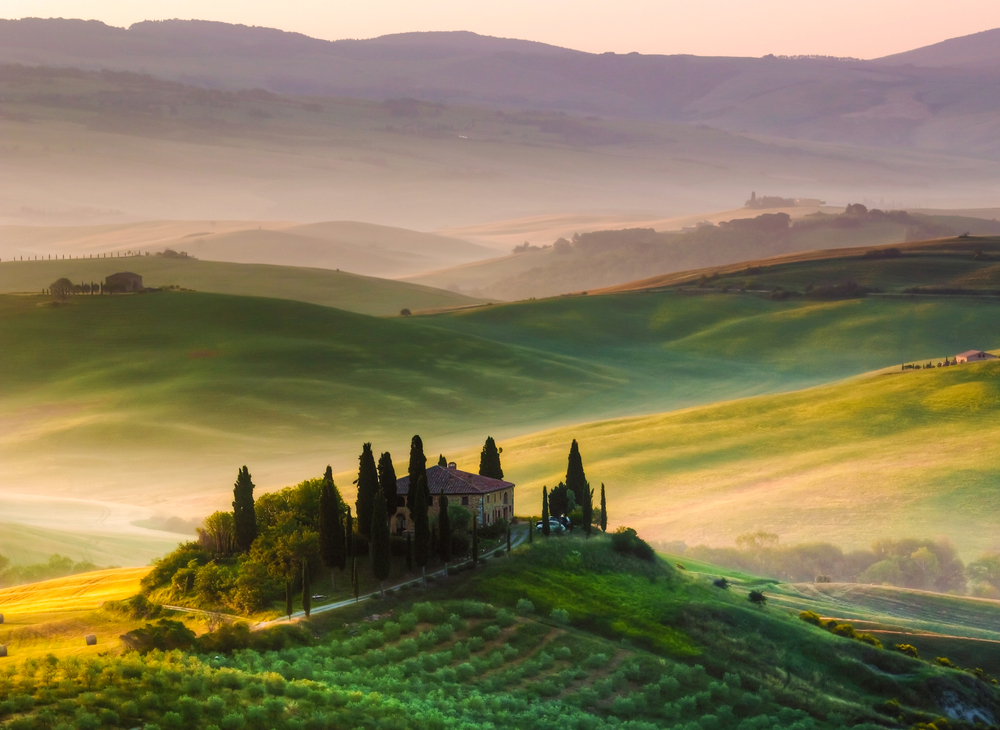
\includegraphics[width=0.5\textwidth]{speed-of-light/tuscany.png}
	\caption{Tuscany Hills}\label{sol:fig:tuscany}
\end{figure}

After Galileo’s first attempt, many ingenious experiments have determined the speed of light with amazing precision (4 parts per billion), including those employing a fast rotating mirror by Albert Michelson, professor at University of Chicago and Nobel Prize in Physics (1907).   

In this lab, you will measure the speed of light with a method similar to Galileo’s but with some helpful improvements: a mirror will replace Galileo’s assistant (eliminating the delay introduced by his reaction time!) and the time of travel will be measured with nanosecond resolution by an extremely fast light detector.

\section{Forming Groups}

Find your group of 2--3 people. You can change groups from week to week, if you'd like.

\begin{steps}
	\item Once you have a group, meet with each other and decide a) what tools you will use to communicate and collaborate, b) when you will meet, c) what you will do when you need to change an agreement, and d) what you will do when a member has a concern about how the group is functioning. \textbf{Record your agreements.}% This part counts as data collection and analysis, so it can be identical in each member's report.}
\end{steps}

\subsection{Team roles}

\begin{steps}
	\item \textbf{Decide on roles} for each group member.
\end{steps}

The available roles are:
\begin{itemize}
	\item Facilitator: ensures time and group focus are efficiently used
	\item Scribe: ensures work is recorded
	\item Technician: oversees apparatus assembly, usage
	\item Skeptic: ensures group is questioning itself
\end{itemize}

These roles can rotate each lab, and you will report at the end of the lab report on how it went for each role. Some members will be holding more than one role. For example, you could have the skeptic double with another role. Consider taking on a role you are less comfortable with, to gain experience and more comfort in that role.

Additionally, if you are finding the lab roles more restrictive than helpful, you can decide to co-hold some or all roles, or think of them more like functions that every team needs to carry out, and then reflect on how the team executed each function.

\subsection{Add members to Canvas lab report assignment group}

\begin{steps}
	\item On Canvas, navigate to the People section, then to the ``Lab 1 Groups'' tab. Find a group that is not yet used, and have each person in your group add themselves to that same lab group.
\end{steps}

This enables group grading of your lab report. Only one person will submit the group report, and all members of the group will receive the grade and have access to view the graded assignment.

\section{The Scientific Cycle\protect\footnote{adapted from Etkina, Planinsic, Van Heuvelen, College Physics, 2nd ed. (2014)}}

One way of describing science is the process of incrementally improving a shared model of how our universe works. In different fields of science, different methods and cycles are used, so there is no ``One True Scientific Method.'' One can still create a model for the process of science, and we describe here one such cycle (the hypothetico-deductive cycle), summarized in Figure~\ref{me:fig:isle}.

In this cycle, there are three types of experiments, each one representing a different stage of the scientific effort. One stage, often started when encountering a novel phenomenon, is the \textbf{observational experiment}. This is an experiment that consists of deciding what to observe and how to observe it, collecting data, finding a pattern, and brainstorming possible explanations for what is observed (also called ``hypotheses'').

Once one has some trial explanations, one can test one or more of those with a \textbf{testing experiment}. Here, one designs a new experimental procedure and uses each hypothesis to predict what will happen. Then the prediction is compared to the procedure's outcome. If they are different, then the hypothesis is judged to be not a helpful explanation for that phenomenon. If they are the same, then it is still helpful. Throughout this stage, one may make various assumptions that would need to be validated, as they can effect the prediction or outcome.

Once a hypothesis has been tested enough for people to find it useful, then it can be applied to solve practical problems, or to determine properties of particular situations, in an ``application experiment.''

\begin{figure}
	\centering
	\includegraphics[width=0.7\textwidth]{ripple-tank/islegraphic.png}
	\caption{A model of the process some scientists go through to create knowledge.\label{me:fig:isle}}
\end{figure}

\section{Application experiment: measure the speed of light}

\subsection{Goal}

Use the kinematic equations to experimentally determine the speed of light produced by a pulsed laser.

\subsection{Available equipment}

\begin{itemize}
	\item Oscilloscope
	\item Pulsed laser
	\item Photodiode
\end{itemize}

\begin{framed}
	\textbf{Warning: Laser Hazard!} The power of our lasers is low enough that the normal human blink reflex is sufficient to protect against incidental eye exposure.
	
	That being said, the following rules reduce the risk of eye exposure to laser light:
	\begin{enumerate}
		\item Do not direct the laser beam into anyone's eye.
		\item Be aware of the laser reflecting off of mirror-like surfaces and where that beam goes.
		\item Turn off the laser when not in use.
		\item Keep the laser pointing horizontally and near the plane of the table, while keep your eyes above that plane.
		\item To determine whether the laser is on, put your hand or a light-colored object in front of the beam, rather than looking into the laser aperture.
	\end{enumerate}
\end{framed}

\begin{framed}
	\textbf{Self-assessment:} To help you improve your scientific abilities, we provide you with self-assessment rubrics.
	A rubric is a scoring system.
	Self-assessment is determining how well you performed a particular task.
	So, these self-assessment rubrics are designed to help you evaluate your performance while you are designing and performing your experiment.
	
	The complete set of rubrics is available in Appendix~\ref{cha:rubrics}.
	In each lab, your report will be assessed using Rubric F, found in Table~\ref{rubric:f}, as well as 5 additional rubric rows listed in that lab.
	Each week, read through these and use them to evaluate your work as you design and perform the experiment.
	Your instructor will use the same rubrics to determine part of your grade for the lab.
\end{framed}	

\subsection{Rubrics to focus on during this experiment:}

See Appendix~\ref{cha:rubrics} for more details.

\begin{itemize}
\item \textbf{A11:} Graph

\item \textbf{D4:} Is able to make a judgment about the results of the experiment

\item \textbf{G1:} Is able to identify sources of experimental uncertainty

\item \textbf{G2:} Is able to evaluate specifically how identified experimental uncertainties affect the data

\item \textbf{G4:} Is able to record and represent data in a meaningful way

\item \textbf{F1:} Is able to communicate the details of an experimental procedure clearly and completely

\item \textbf{F2:} Is able to communicate the point of the experiment clearly and completely

\end{itemize}

\subsection{Speed of light apparatus}

You will use a \textit{time-of-flight} method to measure the speed of light, as illustrated in Figs. \ref{sol:fig:apparatus-sketch}--\ref{sol:fig:apparatus-photo}.  A red laser diode emits periodic flashes of light of very short duration (few $10^{-9}\:$s).  Each pulse of light is directed toward a distant mirror, placed at a distance $L$ from the laser, where it is reflected back toward a light detector (photodiode) located on top of the laser housing. The speed of the light pulse is given by the distance of travel ($D\approx 2L$) divided by the time $t$ required by the pulse to travel to the distant mirror and back:
\begin{equation}\label{sol:eqn:dvt}
v = c = \frac{2L}{t}
\end{equation}
You will measure the distance $L$ with a measuring tape or meter stick, while the time $t$ is measured with the help of an oscilloscope. The electronic circuit driving the laser generates a voltage pulse coincident in time with the firing of the laser flash (yellow line, CH1). A second voltage pulse (blue line, CH2) is produced by the photodiode when hit by the returning light flash. The time difference between these two voltage pulses gives the time of travel $t$.

\begin{figure}
	\centering
	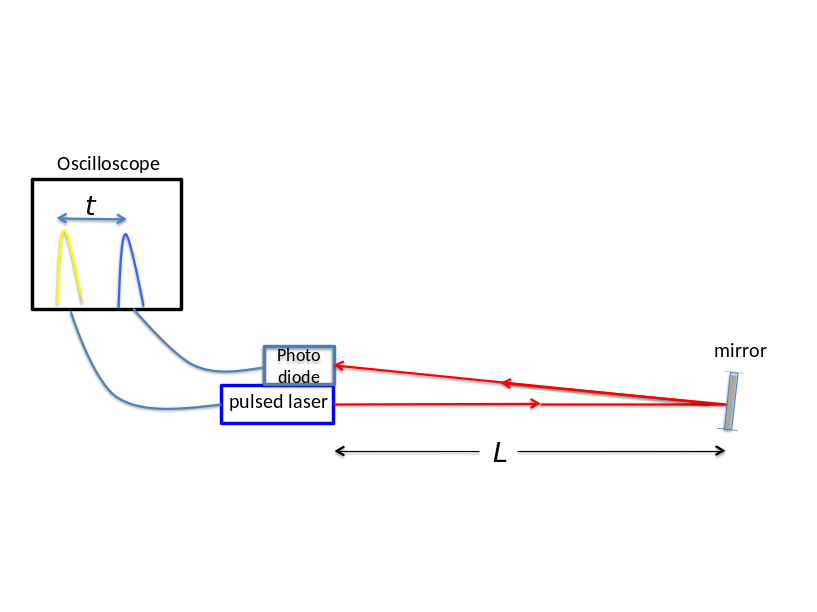
\includegraphics[width=\textwidth]{speed-of-light/apparatus-sketch.png}
	\caption{Sketch of the speed of light apparatus.}\label{sol:fig:apparatus-sketch}
\end{figure}

\begin{figure}
	\centering
	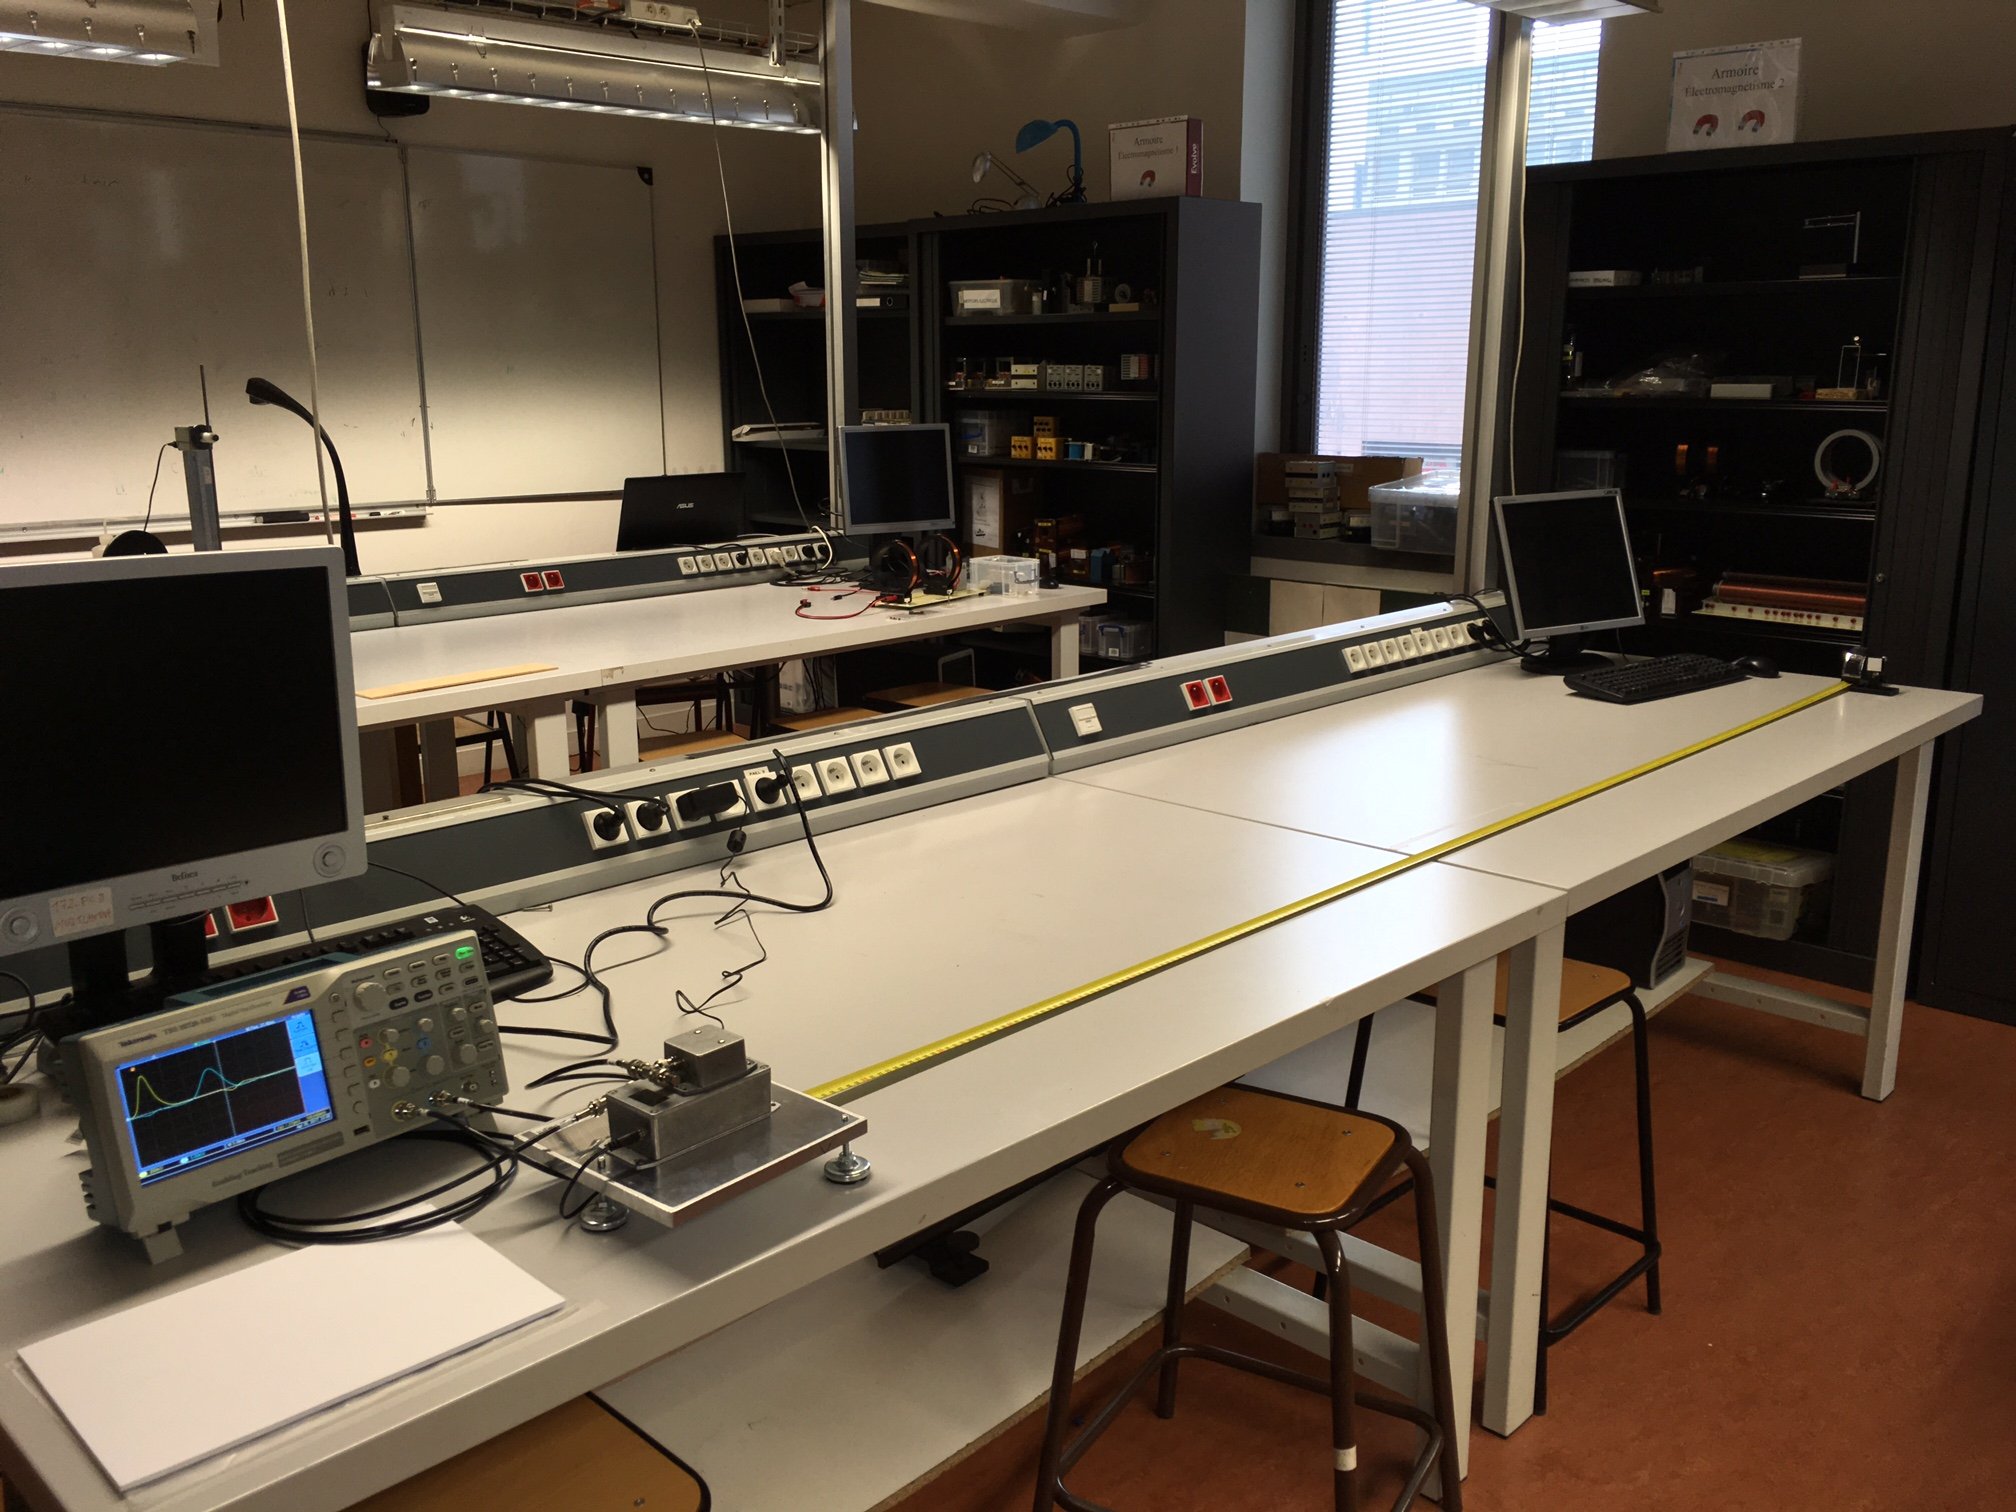
\includegraphics[width=0.8\textwidth]{speed-of-light/apparatus-photo.png}
	\caption{The speed of light setup.}\label{sol:fig:apparatus-photo}
\end{figure}

\subsection{Aligning the mirror}

The alignment of the laser-mirror-photodiode requires a bit of practice but it is not too hard (and is fun!). You will use a sheet of white paper to “catch” the laser spot when doing the alignment.

\begin{steps}
	\item Place the mirror the desired distance from the laser. This is your distance $L$. A useful first distance is 1 meter.
	
	\item Place the white paper at the distance $L$ and see where the laser spot is located. Position the mirror so that the laser spot is approximately at its center (you may have to move the laser base or the mirror vertically.)
	
	\item To catch the reflected laser, slowly move the white paper from the sides (left, right and top with respect to the laser axis) to intercept the laser. Perform this operation with the white paper placed approximately half way between the laser and the mirror. You should find two spots, one of which (the reflected laser beam: “reflected spot”) will disappear when you catch the other (the beam coming directly from the laser: “direct spot”).
	
	\item Once you have identified the reflected spot, move the alignment knobs behind the mirror (slowly, they are very sensitive!) to place it close the direct spot (catching the spots with the white paper will help you during this procedure).  If the reflected spot is too much on the side, you can also rotate the base of the mirror to bring it back along the laser beam axis, and then do the fine adjustments with the mirror alignment knobs.
	
	\item Follow with the white paper the reflected spot back to the laser/photodiode housing. Note that the reflected spot will be quite diffused, particularly for large $L$.
	
	\item By rotating the base of the mirror and/or with small adjustments of the mirror alignment knobs, move the reflected spot so that the photodiode is approximately at its center.  Look at the signal pulse from the photodiode (blue line) and do small adjustment to maximize it so that it is approximately symmetric with a peak height $\ge 15\:$mV.

\end{steps}

\subsection{Observing the signal}

The function of the oscilloscope is to detect a small repeating signal (``oscillation'') and display it in a way useful for analysis. It works at the high frequencies we need (billions of cycles per second, or gigahertz).

\begin{steps}
	\item Be sure that the oscilloscope is setup to display individual pulses (Press “Acquire”, then “Sample”, Figs. \ref{sol:fig:scope-parts} and \ref{sol:fig:scope-average}).

\begin{figure}
	\centering
	\includegraphics[width=0.5\textwidth]{speed-of-light/scope-screen.png}%
	\includegraphics[width=0.5\textwidth]{speed-of-light/scope-commands.png}
	\caption{Left: Oscilloscope screen with Cursor time measurement. Right: Oscilloscope commands.}\label{sol:fig:scope-parts}
\end{figure}

\begin{figure}
	\centering
	\includegraphics[width=0.8\textwidth]{speed-of-light/scope-average.png}
	\caption{Performing Averages with the oscilloscope}\label{sol:fig:scope-average}
\end{figure}

	\item Note the frequency of the periodic flashes as displayed in the lower right corner of the screen. It should be about 100 kHz, since that's the frequency the laser is pulsing at.
	
	\item Expand the time scale by turning the Horizontal Scale knob (see Fig. \ref{sol:fig:scope-parts}, right) and observe that each of these periodic pulses is actually two, closely spaced pulses (Fig. \ref{sol:fig:scope-parts}, left).
	
\end{steps}

The first pulse (yellow line) corresponds to the time when the laser emits the flash, the second pulse (blue line) corresponds to the time of arrival of the light flash at the photodiode.

\subsection{Doing one measurement}

Here you'll actually do a measurement of the speed of light by measuring the distance and time duration and applying Equation\ \ref{sol:eqn:dvt}.

\subsubsection{Measuring distance}

\begin{steps}

	\item With the laser aligned and both pulses visible, measure the mirror distance $L$.

\end{steps}
	
A measurement of a physical quantity is not useful without an estimate of the uncertainty of the measurement.

\begin{steps}
	\item Skim the introduction and Section \ref{unc:sec:types} of Appendix \ref{cha:uncertainty}.
	
	\item Identify some possible sources of uncertainty for the mirror distance measurement. \textbf{Record your answers.}

	\item For each source of uncertainty, decide on the type of uncertainty --- instrumental or random. \textbf{Record your answers.}
	
	\item For each source of uncertainty, estimate the amount of uncertainty. \textbf{Record your answers.}
	
	\item For this measurement, pick the greatest uncertainty from the various sources and ignore the others. Treat this as the uncertainty of this measurement. \textbf{Record your final determination of $L$ and uncertainty $\delta L$.} Express this as $L \pm \delta L$, for example $L = 1.02 \pm 0.01\:$meters.

\end{steps}

\subsubsection{Measuring time}

\begin{steps}

	\item To optimally measure the difference in time between the two pulses, maximize the resolution of the time (Horizontal) scale while keeping both pulses in the screen. The resolution is displayed in the lower middle of the screen, labeled ``M''. Typically you will choose a $5\:$ns/division or $10\:$ns/division in the horizontal scale. Place the source laser pulse (CH1, yellow line) as far left as possible using the Horizontal Position knob so that the full horizontal scale can be used for the measurements.
	
	\item Optimize the photodiode pulse (CH2, blue line) by aligning the laser spot on the photodiode. The resulting pulse should be approximately symmetric with a peak height $\ge 15\:$mV. \textit{Note: always keep the vertical scale of Channel 2 at $\ge 5\:$mV/division, as shown in the lower left marked ``2''.}
	
\end{steps}

Next you will set up the oscilloscope to perform the average of 128 pulses, which will provide improved accuracy in the determination of the position of the pulses.

\begin{steps}
	\item To set the oscilloscope for the average measurement (Fig. \ref{sol:fig:scope-average}), press “Acquire”, then press “Average” and rotate the Multipurpose knob till the number 128 (i.e. average of 128 pulses) is highlighted, and press the Multipurpose knob to select. Press “Menu off” to eliminate the Menu from the screen.
	
\end{steps}

Next you will use the time cursors to measure the time difference $t$ between the peaks of the two pulses.

\begin{steps}
	
	\item Press “Cursor” (Fig. \ref{sol:fig:scope-parts}, right). Check that cursor “Type” is “Time”, then press “Cursor 1” in the Cursor Menu and move the cursor by turning the Multipurpose knob so that it coincides with the peak of the source pulse. Press “Cursor 2” and move the cursor until it coincides with the peak of the detector pulse. The time difference between the two cursors (corresponding to the time of travel $t$) will be displayed as “$\Delta$ .. ns” in the Cursor Menu (third tab from the top). \textbf{Record your measured time difference.}
	
	\item Identify the sources of uncertainty, estimate each of them, choose the largest, and \textbf{record your time difference $t$ and its uncertainty $\delta t$.}

	\item Use Equation \ref{sol:eqn:dvt} to find your measurement of the speed of light $v_c$.

	\item To find the uncertainty in your measured $v_c$, we must propagate the uncertainty from $L$ and $t$. Since the formula involves division of these two variables, use Equation \ref{unc:mult} to find $\delta v_c$. \textbf{Record your calculation of $v_c \pm \delta v_c$}

\end{steps}

It is okay if this measurement is much different from the standard value of $c \approx 3 \times 10^8\:$m/s. We will examine a possible reason for this in the next section. It should be within a factor of 2 or so at this point. If not, check with your instructor.

\begin{steps}

	\item Press “Acquire”, then “Sample”. This will return the oscilloscope to display individual pulses.

\end{steps}

\section{Checking assumptions}

In our model of the scientific cycle, sources of uncertainty are ones that are quantifiable --- we can estimate the effect and include it as an interval within which we are confident. We use \textit{assumption} to mean things that we are assuming are true that, if not true, would change our result in ways that we cannot or are not estimating. Some assumptions are more about troubleshooting --- for example, we assume that the oscilloscope is working as expected. Others are about our measurement technique. For example, there is a vertical distance between the laser source and the detector. This means that the path the light travels is not simply $2L$.

\begin{steps}
	
	\item By assuming the path the light travels is $2L$, will you over- or under-estimate value of $c$, compared with using a more accurate length? \textbf{Record your answer.}
	
	\item Estimate how much your measurement of the speed of light will change if you use the correct value for the return path (note: the distance between the laser and the photodiode is $4\:$cm). For simplicity, make your estimate only for the measurement where the mirror was at the maximum distance. Do you think this is a small or large effect? \textbf{Record your answers.}
	
\end{steps}

Another assumption is that the lag time from detector to oscilloscope and from source to oscilloscope is the same. That is, the time difference recorded in the oscilloscope includes the time for the signals from the laser and detector to reach it. Since we are talking about time differences on the  order of nanoseconds, small differences in cable length, for example, could change things.

This fixed difference in length $d_e$ is the same no matter the mirror distance $D=2L$. In fact, it should be the same error in length every time. So the recorded time difference $t$ would actually be 
\begin{eqnarray}
\textrm{total distance} &=& vt \\
2L + d_e &=& v t \\
2L &=& v t - d_e
\end{eqnarray}

Notice that the last equation is in the same form as that of a straight line, $y = mx + b$. So if we take a series of measurements of $t$ for different distances $2L$, and plot $2L$ vs. $t$, then the slope of the graph will be the speed of light $v$, and that effective length difference $d_e$ will be the $y$-intercept.

\begin{steps}

	\item Measure the time difference for at least 5 different mirror distances, \textbf{recording your measurement in a table}, including the distance $L$ between the laser and the mirror that you have measured with the measuring tape or meter stick. See Table \ref{sol:tab:data} for a sample table format.

\begin{table}
	\centering
	\begin{tabular}{|c|c|c|}
		\toprule
		length (m) & distance $= 2L$ (m) & time ($10^{-9}\:$s) \\
		\midrule
		\ldots & \ldots & \ldots \\
		\bottomrule
	\end{tabular}
	\caption{Sample data collection table.}\label{sol:tab:data}
\end{table}

	\item Once your measurements are completed, graph the data of your table in a plot with time of travel $t$ in the horizontal axis and distance of travel ($D = 2L$) in the vertical axis.
	
	\item To determine the speed of light $c$, fit your data with a line (e.g. with Excel by displaying your data with Scatter, and then using Trendline;  select 'Display Equation on Chart' in Trendline Options). The slope of the line will be your estimate of the speed of light. (NOTE: pay attention to the units). \textbf{Take a screenshot of your graph for your report.}
	
\end{steps}
	
In this case, to determine the uncertainty, you will not use the uncertainty of each individual point. Instead, you will use the coefficient of determination, $r^2$, which is given by your plotting program, along with the number of data points you took, $N$, to find the uncertainty, which is the standard error $SE$ of the slope $m$, given as
\begin{equation}\label{sol:eqn:sem}
SE(m) = m \sqrt{\frac{1-r^2}{r^2 (N-2)}}
\end{equation}

\begin{steps}

	\item Find the uncertainty in the speed of light measurement using Equation \ref{sol:eqn:sem}. \textbf{Record your new determination of $c$, with its uncertainty.}
	
	\item Compare your result with the known value of the speed of light, $299\:792\:458\:$m/s. To compare, use the $t'$ statistic as described in Appendix \ref{unc:sec:comparing}.

\end{steps}

\section{Revisiting Galileo's technique}

\begin{steps}
	
	\item Measure your reaction time with a stopwatch (highly likely you have one in your cell phone, or ask the instructor if you need one).  Start-stop the stopwatch and record the time. Take 10 measurements and calculate their average as an estimate of your reaction time.\textbf{Record your results.}
	
	\item Now, imagine you  climb on top of a hill in beautiful Tuscany and shoot a laser pulse (by pressing a button at the same time of the start in the stopwatch) towards a mirror placed $2\:$km away. You press the stop in the stopwatch as soon as you see the returning laser pulse. Would you be able to measure the speed of light? (Calculate the time of travel of the laser pulse and compare it with your reaction time). \textbf{Record your answer and calculation.}
	
	\item At what distance should the mirror be placed for you to be able to measure the speed of light (say with a 20\% uncertainty) using the stopwatch? \textbf{Record your answer.}

\end{steps}

\section{Group dynamics}

\begin{steps}
	\item Write a 100--200 word paragraph reporting back from each of the four roles: facilitator, scribe, technician, skeptic. Where did you see each function happening during this lab, and where did you see gaps? What successes and challenges in group functioning did you have? What do you want to do differently next time?
\end{steps}

\section{Report checklist and grading}

The lab grade consists of 3 points for each of seven scientific ability rubric rows (the 5 listed above, as well as F1 and F2, applied to the entire report), 3 points for attendance and participation, and 6 points for providing evidence in the lab report of completing all steps of the lab, including answering every question, for a total of 30 points.
\chapter{Local Gravitational Field}

One of Newton's revelations was that physical laws that governed the movement of objects near Earth also predicted the movements of objects in the sky.
The apocryphal story of an apple falling on Newton's head brings to mind the mechanism of gravity --- the phenomenon of massive objects attracting each other.
In this lab, you will measure the strength that gravity has where we are, near the Earth's surface. This measurement might also enable us to learn more about the mass of the Earth itself in a future lab.

\section{Learning goals}

\begin{itemize}
	\item Understand Newton's law of universal gravitation and its linear approximation
	
	\item Identify sources of statistical and systematic error
	
	\item Demonstrate an ability to make careful measurements
	
	\item Demonstrate proficiency in basic calculations and plotting
	
	\item Explain the importance of repeated measurements and sufficiently large datasets
\end{itemize}

\subsection{Team roles}

\begin{steps}
	\item \textbf{Decide on roles} for each group member.
\end{steps}

The available roles are:
\begin{itemize}
	\item Facilitator: ensures time and group focus are efficiently used
	\item Scribe: ensures work is recorded
	\item Technician: oversees apparatus assembly, usage
	\item Skeptic: ensures group is questioning itself
\end{itemize}

These roles can rotate each lab, and you will report at the end of the lab report on how it went for each role. Some members will be holding more than one role. For example, you could have the skeptic double with another role. Consider taking on a role you are less comfortable with, to gain experience and more comfort in that role.

Additionally, if you are finding the lab roles more restrictive than helpful, you can decide to co-hold some or all roles, or think of them more like functions that every team needs to carry out, and then reflect on how the team executed each function.

\subsection{Add members to Canvas lab report assignment group}

\begin{steps}
	\item On Canvas, navigate to the People section, then to the ``L2 G Field [number]'' tab. Find a group that is not yet used, and have each person in your group add themselves to that same lab group.
\end{steps}

This enables group grading of your lab report. Only one person will submit the group report, and all members of the group will receive the grade and have access to view the graded assignment.

\section{Scientific Background}

\subsection{The gravitational field strength and Newton's second law}

The force of gravity, $F$, between two objects with mass $m_1$ and $m_2$ and whose centers are separated by a distance $R$ is given by Newton's law,
\begin{equation}\label{lg:eq:newtons}
 F_\textrm{gravity} = G \frac{m_1 \: m_2}{r^2} \,,
\end{equation}
where the Newtonian constant of gravitation $G = 6.67408(31) \times 10^{-11} \: \textrm{m}^3 \: \textrm{kg}^{-1} \: \textrm{s}^{-2}$. Astronomers apply Newton's law to infer fundamental information about astrophysical objects, for example the mass of binary stars. Indeed, this is one of the most common methods by which astronomers ``weigh'' astrophysical objects, including the Earth itself. For measuring the force acting on an object of mass $m$ that is affected predominantly by the Earth's gravity, the force acting on it would be
\begin{equation}\label{lg:eq:fearth}
 F_\textrm{Earth} = \frac{G M_\Earth}{(R_\Earth + h)^2} m
\end{equation}
where $M_\Earth$ and $R_\Earth$ are the mass and radius of the Earth, respectively, and $h$ is the height above the Earth.

For objects near the Earth's surface, where $h$ is much less than $R_\Earth$, $h$ can be treated as zero, resulting in a constant gravitational force, with Equation~\ref{lg:eq:fearth} reducing to
\begin{equation}\label{lg:eq:fearthred}
F_\textrm{Earth} = \frac{G M_\Earth}{(R_\Earth)^2} m \,.
\end{equation}
Notice that on the right-hand-side of this equation, the only variable is the mass. The others, together, constitute the \textit{strength of the local gravitational field}, $g$ (sometimes pronounced ``little g''). So our simplified equation is
\begin{equation}\label{lg:eq:fegm}
 F_\textrm{Earth} = g m \,,
\end{equation}
where we have made the substitution
\begin{equation}\label{lg:eq:g}
g = \dfrac{G M_\Earth}{(R_\Earth)^2} \, .
\end{equation}
Notice that we have taken a complicated inverse square equation (Equation~\ref{lg:eq:fearth}) and
converted it to a much simpler one (Equation~\ref{lg:eq:fegm}). This process is called \textit{linearization} and is a
trick astronomers often use to make calculations more manageable. You will encounter
this technique throughout this and other PHSC courses.

We see from Equation~\ref{lg:eq:g} that if we can make accurate measurements of $g$, $G$, and $R_\Earth$, we can calculate the mass of the Earth. We'll look up $R_\Earth$ online, and next week we will measure $G$. To find $g$, we note that Newton's second law of motion states that the acceleration $a$ of an object is directly proportional to the net force $F_\textrm{net}$ acting on it and inversely proportional to its mass, $m$, or, more succinctly and slightly rearranged,
\begin{equation}
 F_\textrm{net} = m a \,.
\end{equation}
If the Earth's gravity is the only force acting on our object, then $F_\textrm{net} = F_\textrm{Earth}$, and substituting Equation~\ref{lg:eq:fegm}, we find that
\begin{equation}
 g m = m a \,,
\end{equation}
and thus, simplifying,
\begin{equation}
 a = g \,.
\end{equation}
So, the acceleration of an object that is subject only to the Earth's gravity is equal to the local gravitational field strength. If we can measure the acceleration, then we can find $g$, and get one step closer to determining the mass of the Earth.

\subsection{Constantly accelerated motion}

If an object is subject to a constant force, then according to Newton's second law, it undergoes constant acceleration. If an object undergoes constant acceleration $a$, and we know the object's initial position $x_0$ and velocity $v_0$, then after a time duration $t$, we can derive using calculus that the object's position $x$ and velocity $v$ are given by
\begin{equation}\label{lg:eq:x-const-a}
 x = x_0 + v_0 t + \frac{1}{2} a t^2
\end{equation}
and
\begin{equation}
 v = v_0 + a t \,.
\end{equation}

\section{Application experiment: determine $\bm{g}$ on the Earth's surface}

\subsection{Goal}

Determine $g$ near the Earth's surface by finding the acceleration of an object undergoing freefall (no substantial forces other than gravity) using two different methods.

\subsection{Rubrics to focus on}

See Appendix~\ref{cha:rubrics} for more details.

\begin{itemize}
	\item \textbf{D4:} Is able to make a judgment about the results of the experiment

	\item \textbf{D5:} Is able to evaluate the results by means of an independent method

	\item \textbf{G1:} Is able to identify sources of experimental uncertainty
	
	\item \textbf{G2:} Is able to evaluate specifically how identified experimental uncertainties affect the data
	
	\item \textbf{G4:} Is able to record and represent data in a meaningful way
	
	\item \textbf{F1:} Is able to communicate the details of an experimental procedure clearly and completely
	
	\item \textbf{F2:} Is able to communicate the point of the experiment clearly and completely
	
\end{itemize}

\subsection{Available equipment}

\begin{itemize}

	\item Stopwatch
	\item Dense object to drop
	\item Meter stick
	\item Camera (including the one on your phone)
	\item Computer with Tracker\footnote{Open Source Physics Tracker can be downloaded from \url{https://physlets.org/tracker} and is also installed on the lab computers.} installed.

\end{itemize}

\subsection{Method 1: freefall time}

\begin{steps}
	\item Drop the object from a known height and measure the time to fall with a stopwatch. Do this as many times as makes sense to you.
	
	\item List the sources of uncertainty and determine whether each is a random uncertainty or an instrumental uncertainty.
	
	\item Calculate the average fall time.
	
	\item Calculate the standard deviation of the average fall time (using Equation~\ref{unc:eq:stdevmean}), and report the latter as the uncertainty in the average fall time.
	
	\item Use the average fall time and the initial position and velocity of the object to calculate the acceleration.
	
	\item Propagate the uncertainty in the time and position to find the uncertainty of your measured acceleration (see Section~\ref{unc:sec:prop})
	
	\item Report the acceleration found by this method as ``value $\pm$ uncertainty [units]''. For example, $9.73 \pm 0.04\:$m/s$^2$.
\end{steps}

\subsection{Method 2: Video tracking}

It is helpful to use two methods to find the same quantity, so that mistakes or incorrect assumptions made in one method do not carry over to the other, and are thus more likely to be detected. In this method, you will record a video of an object falling, make a position vs. time plot, and fit the constant acceleration equation (Equation~\ref{lg:eq:x-const-a}). You will use a computer program to make this analysis easier.

\subsubsection{Record the video}

\begin{steps}
	\item Find a good object to drop. It should be dense enough to not be slowed down significantly by air resistance.
	
	\item Using the camera on one of your group member's phones, record a video of the object falling.
	
	Here are some tips to get a quality video:
	\begin{itemize}
		\item Include an object of known length in the shot, at the same distance from the camera as the falling object. This gives a reference length, so that you can find how each camera pixel scales to the physical situation.
		
		\item Avoid parallax error by having the object be at about the same distance from the camera throughout the fall. Having the camera be farther away can help. Also, you can ensure that the top and the bottom of the fall are the same distance from the camera.
		
		\item Hold the camera steady.
	\end{itemize}

	\item Record that video and transfer the video to a computer that has Tracker installed.
\end{steps}

\subsubsection{Importing the data into Tracker}

In this part, you'll use Tracker to record the position of the object at each timestep. To do this, you'll need to tell it what direction ``down'' is in, what the scale of the image is, and when time $t=0$ is. Then you'll record the positions, find out what parameters best fit the curve that is produced, and use those to find the acceleration.

\begin{steps}
	\item Open Tracker on a computer. You can install it on your own computer by visiting \url{https://physlets.org/tracker}.
	
	\item Optionally, watch this 3-minute tutorial on how to use Tracker: \url{https://www.youtube.com/watch?v=n4Eqy60yYUY}
	
	\item In Tracker, open your video.
	
	\item \textbf{Find frame when zero time is.} Move the slider below the video to the right to advance the frames until you find the first one in which the object is falling. Record that start frame number, which is found to the left of the slider bar in red.
	
	\item \textbf{Find the last relevant frame.} Keep moving the slider to the right until you find the last frame before the object hits the floor. Record that end frame number.
	
	\item To \textbf{tell Tracker about these frames}, click the 5th icon from the left on the toolbar above the video (``Clip settings'') and enter the start frame and end frame.
	
	\item \textbf{Tell Tracker how long things are.} In astronomy applications, this is known as the ``pixel scale''. Here we can just draw a line on the frame and tell Tracker how long that line is in real life. Click the 6th icon from the left (blue, with a ``10'') and select \texttt{New} $\rightarrow$ \texttt{Calibration Stick}. Shift-click to mark each end of your known length, and type in your known length, with units in the box that appears along the stick. Use ``m'' for meters.
	
	\item \textbf{Align the coordinate system.} In the toolbar, click the 7th icon from the left (magenta crossed lines). Click and drag the coordinate system's origin (the intersection of long lines) to the location of the object in the start frame.
	
	\item \textbf{Check to see if the camera was tilted.} Advance the video to see if the object moves along an axis. If it goes off at an angle, the camera was tilted compared to the direction of motion. In this case, rotate the coordinate system to align with the motion by clicking and dragging the small line that crosses one of the axes.
	
	\item \textbf{Tell Tracker where the object is in every frame.}
	\begin{enumerate}
		\item In the toolbar, click \texttt{Create} $\rightarrow$ \texttt{Point Mass}.
		\item Ensure the slider is at the start frame.
		\item Shift-click on the object. Notice that the frame advances to the next one automatically.
		\item Continue to shift-click to mark the object's position throughout the duration.
	\end{enumerate}
\end{steps}

\subsubsection{Analysis}

\begin{steps}
	\item \textbf{Ensure the correct axis is selected for analysis.} Look at the plot to the right of the video. If there is not a smooth-ish curved line, click on the axis label ``x (m)'' and choose instead ``y (m)''.
	
	\item In the drop-down menu, select \texttt{View} $\rightarrow$ \texttt{Data Tool (Analyze...)}.
	
	\item In the window that appears, above the plot, click \texttt{Analyze} $\rightarrow$ \texttt{Curve Fits}.
	
	\item Notice that Eq.~\ref{lg:eq:x-const-a}, which describes freefall, is a quadratic equation, which means the shape is a parabola. For ``Fit Name'', choose ``Parabola'' from the drop-down menu.
	
	\item Use the Fit Equation and Parameter Values, comparing with Equation~\ref{lg:eq:x-const-a}, to find the acceleration $a$, and thus the gravitational field strength $g$.
	
	\item To get an uncertainty for this value, use the ``rms dev'' value, which describes the average deviation of the fit equation from the points, divide that by the average (mean) position, and multiply that by your value for the acceleration. You can find the mean position by selecting \texttt{Analyze} $\rightarrow$ \texttt{Statistics} and reading above the data table column.
\end{steps}

\subsection{Comparing the methods, final determination of $\bm{g}$}

\begin{steps}
	\item Compare the values of $g$ from the two methods using the $t'$ statistic as described in Appendix~\ref{unc:sec:comparing}.
	
	\item Use that comparison and your assessment of which method had fewer questionable assumptions to decide on your final answer for $g$ (including an uncertainty). How close is it to the average $g$ described, for example, on Wikipedia?
\end{steps}

\section{Group dynamics}

\begin{steps}
	\item Write a 100--200 word paragraph reporting back from each of the four roles: facilitator, scribe, technician, skeptic. Where did you see each function happening during this lab, and where did you see gaps? What successes and challenges in group functioning did you have? What do you want to do differently next time?
\end{steps}

\section{Report checklist and grading}

The lab grade consists of 3 points for each of seven scientific ability rubric rows (the 5 listed above, as well as F1 and F2, applied to the entire report), 3 points for attendance and participation, and 6 points for providing evidence in the lab report of completing all steps of the lab, including answering every question, for a total of 30 points.
%\chapter{Using light waves to measure small distance changes (Michelson interferometer)}

\section{Introduction}

With the basic properties of waves and wave interference established (via the ripple tank) and the same behavior
demonstrated in light (via the laser-based modern version of Young's double slit experiment) we are now finally ready to
look at a Michelson interferometer. This technology is the basis of the LIGO experiment. You may want to refer back to
the introduction of Lab~\ref{cha:ripple-tank} to remind yourself of some details. LIGO itself is a large experiment that has
been constructed over several decades of work and technology development, and so is many orders of magnitude more
precise and sensitive than what we can do in an hour on a lab bench. Nevertheless, the basic principles are the same.

%\section{Learning Goals}

\section{Team roles}

\begin{steps}
	\item \textbf{Decide on roles} for each group member.
\end{steps}

The available roles are:

\begin{itemize}
	\item Facilitator: ensures time and group focus are efficiently used
	\item Scribe: ensures work is recorded
	\item Technician: oversees apparatus assembly, usage
	\item Skeptic: ensures group is questioning itself
\end{itemize}

These roles can rotate each lab, and you will report at the end of the lab report on how it went for each role. If you have fewer than 4 people in your group, then some members will be holding more than one role. For example, you could have the skeptic double with another role. Consider taking on a role you are less comfortable with, to gain experience and more comfort in that role.

Additionally, if you are finding the lab roles more restrictive than helpful, you can decide to co-hold some or all roles, or think of them more like functions that every team needs to carry out, and then reflecting on how the team executed each function.

\section{Add members to Canvas lab report assignment group}

\begin{steps}
	\item On Canvas, navigate to the People section, then to the ``Lab 3 Groups'' tab. Find a group that is not yet used, and have each person in your group add themselves to that same lab group.
\end{steps}

This enables group grading of your lab report. Only one person will submit the group report, and all members of the group will receive the grade and have access to view the graded assignment.

\section{Observation experiment: demonstration of the interferometer}

\subsection{Goal}

Observe the flow of light in the Michelson interferometer simulation.

\subsection{Available equipment}

\begin{itemize}
	\item A virtual Michelson interferometer found at \url{https://www.geogebra.org/m/msfpudej}
	\begin{itemize}
		\item Note: in the sim, do not zoom in and out by scrolling --- when this happens, the coordinate system appears to shrink and expand, leading to the mirrors seeming to move in space.
	\end{itemize}
\end{itemize}

\subsection{Rubrics to be assessed for this section}

None.

\section{Steps}

\begin{steps}
	\item Load the virtual apparatus at the address listed in the available equipment section.
	
	\item Click the refresh button in the simulation, to the right of the Zeit slider. This fixes a bug where the green wave does not fully display.

	\item Slide Zeit (German for "time") to the left to equal 0. Uncheck "Weg Spiegel 1" (wave path 1)
\end{steps}

This is the Michelson interferometer, invented by Albert Michelson, a physicist whose family immigrated to the USA from Poland when he was 2 years old. He grew up in mining camps in California and Nevada and went on to found the physics department here at UChicago. Let's walk through the operation of the interferometer step by step. A schematic of the setup with parts labeled is found in Figure\ \ref{mir:fig:setup}.

\begin{figure}
	\centering
	\includegraphics[width=\textwidth]{michelson-interferometer-remote/michelson-setup-geogebra}
	\caption{Diagram of the Michelson interferometer simulation with parts labeled.}\label{mir:fig:setup}
\end{figure}

\begin{steps}
	\item Select "Animation" and watch as the wave leaves the laser source and select it again to pause as the wave encounters the beam splitter.
\end{steps}

The beam splitter is a device that reflects some of the beam and transmits the rest. This one is a 50/50 beam splitter, so it splits the beam into equal parts.

\begin{steps}
	\item Select "Animation" again to watch the reflected part of the beam travel until it reaches the output/viewing screen. You'll watch the transmitted part of the beam at a later step. For now it is not displayed. \textit{If the reflected beam does not appear, refresh the animation using the circular arrow button to the right of the Zeit slider.}
\end{steps}

This reflected beam travels to the stationary mirror a distance $d_2$, reflects from that mirror, travels directly through the beam splitter on the way back, and exits the device to be seen on the viewing screen. (we ignore the part that is reflected when it strikes the beam splitter on the way back). The arrow that appears at the output represents the phase of the wave that is passing that point. For example, when the wave is cresting, the arrow points up, and when the wave is at a trough, the arrow points down.

\begin{steps}
	\item Move Zeit back to zero. Check the box for Weg Spiegel 1 and uncheck Weg Spiegel 2. Watch the animation again to follow the path of the beam that is initially transmitted through the beam splitter.
\end{steps}

This beam strikes the mirror at $d_1$, which is movable using the slider on the left or by typing in the desired distance. The typing field accepts numbers with precision up to 4 decimal places.

\begin{steps}
	\item Move Zeit back to zero, check both boxes, and watch the beams overlap with each other at the output.
\end{steps}

In this way the original beam of light splits, and portions of the resulting beams are brought back together to interfere with each other. The black arrow represents the sum of the two waves. The direction is the phase and the length is proportional to the amplitude of the resulting wave.

\section{Testing experiment: testing the theory of wave interference}

\subsection{Goal}

Test if the theory of wave interference and path length difference predicts the correct behavior in the situation of the Michelson interferometer. This theory states that for two different sources of waves that are of the same, single wavelength, and which started out in phase, then constructive interference occurs at a location when the difference in travel distances (path lengths) between the two sources is an integer number of wavelengths. Destructive interference occurs when the path length difference is a half-integer, for example 0.5, 1.5, or 2.5 wavelengths.

\subsection{Available equipment}

\begin{itemize}
	\item A virtual Michelson interferometer as in the previous experiment.
\end{itemize}

\subsection{Rubrics to be assessed for this section}

\begin{itemize}
	\item \textbf{C4:} Is able to make a reasonable prediction based on a hypothesis
	\item \textbf{C7:} Is able to decide whether the prediction and the outcome agree/disagree
	\item \textbf{F1:} Is able to communicate the details of an experimental procedure clearly and completely
	\item \textbf{F2:} Is able to communicate the point of the experiment clearly and completely
\end{itemize}
See Appendix~\ref{cha:rubrics} for details.

\subsection{Suggestions for your experiment}

\begin{itemize}
	\item Ensure that all group members are familiar with how path length difference results in constructive and destructive interference.
	
	\item Examine the geometry of the setup to determine the path length of the beam that travels through each arm of the interferometer.
	
	\item Develop a specific prediction of what setting combinations of wavelength and mirror distance will result in different observable interference effects.
	
	\item Note that in the simulation, you can type in a mirror distance $d_1$ with a precision of 4 decimal places. Press enter after typing it in to save it and have the result displayed.
\end{itemize}

\subsection{Items to include in your report}

Relevant rubric rows from Appendix~\ref{cha:rubrics} are listed in parentheses.

\begin{enumerate}
	\item Clear statement of the hypothesis you are testing (C1, not assessed) [2 pts]
	\item Prediction that follows from the hypothesis, along with justification (C4) [2 pts]
	\item Description of experimental procedure to produce outcome (F1) [2 pts]
	\item Determination of how much the prediction agrees with the outcome (C7) [2 pts]
	\item A discussion of the findings of the experiment and why it's helpful (for you and/or for science) (F2) [2 pts]
\end{enumerate}

\section{Application experiment: measuring length changes with the interferometer}

\subsection{Goal}

The Michelson interferometer is used for LIGO since gravitational waves create very small vibrations in spacetime as they pass. These vibrations literally alter the distance between the beam splitter and mirror along one axis. This MI simulates this with a movable mirror. Using this virtual MI, \textbf{develop a procedure} to determine the change in mirror distance $d_1$ if given the image of the black arrow as displayed on the screen (the arrow's length is proportional to the brightness at that location and moment). \textbf{Demonstrate this procedure} with an example initial and final mirror position.

\textbf{Determine how small} a change in the mirror distance you can measure using your procedure (the \textit{resolution} of the instrument. \textbf{Identify methods} to improve this resolution. 

\subsection{Available equipment}

\begin{itemize}
	\item A virtual Michelson interferometer as in the previous experiment.
\end{itemize}

\subsection{Rubrics to be assessed for this section}

\begin{itemize}
	\item \textbf{D2:} Is able to design a reliable experiment that solves the problem
	\item \textbf{G2:} Is able to evaluate specifically how identified experimental uncertainties affect the data
	\item \textbf{G3:} Is able to describe how to minimize experimental uncertainty and actually do it
	\item \textbf{F1:} Is able to communicate the details of an experimental procedure clearly and completely
	\item \textbf{F2:} Is able to communicate the point of the experiment clearly and completely
\end{itemize}

See Appendix~\ref{cha:rubrics} for details.

\subsection{Suggestions for your experiment}

\begin{itemize}
	\item Remember that the laser wavelength $\lambda$ and the mirror distances are given in micrometers ($\mu$m). This makes it an infrared laser.
	
	\item Decide how you will measure the black arrow's length. This can many methods, for example holding up a ruler to the screen or taking a screenshot and measuring the pixel length in an image analysis program like ImageJ.
	
	\item Note that in the simulation, you can type in a mirror distance $d_1$ with a precision of 4 decimal places. Press enter after typing it in to save it and have the result displayed.
\end{itemize}

\subsection{Items to include in your report}

Relevant rubric rows from Appendix~\ref{cha:rubrics} are listed in parentheses.

\begin{enumerate}
	\item Description of procedure to use image of black arrow to determine the change in mirror distance $d_1$ (D2, F1) [2 pts]
	\item Demonstration of this procedure [2 pts]
	\item Determination of measurement resolution (G2) [2 pts]
	\item Identification of ways to improve this resolution (G3) [2 pts]
	\item A discussion of the findings of the experiment and why it's helpful (for you and/or for science) (F2) [2 pts]
\end{enumerate}

\section{Group functioning}

\begin{steps}
	\item A 100--200 word reflection on group dynamics. Address the following topics: who did what in the lab, how did you work together, how group roles functioned, what successes and challenges in group functioning did you have, and what do you want to continue doing or do differently?
\end{steps}

\section{Individual homework}

\begin{enumerate}
	\item If you were to add a mirror between the beam splitter and the movable mirror, such that the light struck the movable mirror, then our new mirror, then back to the movable mirror, then back to the beam splitter, how would this change the resolution of your measuring device from the application experiment, if at all?
	
	\item Given the resolution of your instrument that you found in the application experiment, what are examples of objects at that length scale that you would be able to use this to measure with 1\% accuracy? You can use this website as a starting point: \url{https://htwins.net/scale2/}
\end{enumerate}
%\chapter{Using light waves to measure small distance changes (Michelson interferometer)}

\section{Introduction}

With the basic properties of waves and wave interference established (via the ripple tank) and the same behavior
demonstrated in light (via the laser-based modern version of Young's double slit experiment) we are now finally ready to
look at a Michelson interferometer. This technology is the basis of the LIGO experiment. You may want to refer back to
the introduction of Lab~\ref{cha:ripple-tank} to remind yourself of some details. LIGO itself is a large experiment that has
been constructed over several decades of work and technology development, and so is many orders of magnitude more
precise and sensitive than what we can do in an hour on a lab bench. Nevertheless, the basic principles are the same.

%\section{Learning Goals}

\section{Team roles}

\begin{steps}
	\item \textbf{Decide on roles} for each group member.
\end{steps}

The available roles are:

\begin{itemize}
	\item Facilitator: ensures time and group focus are efficiently used
	\item Scribe: ensures work is recorded
	\item Technician: oversees apparatus assembly, usage
	\item Skeptic: ensures group is questioning itself
\end{itemize}

These roles can rotate each lab, and you will report at the end of the lab report on how it went for each role. If you have fewer than 4 people in your group, then some members will be holding more than one role. For example, you could have the skeptic double with another role. Consider taking on a role you are less comfortable with, to gain experience and more comfort in that role.

Additionally, if you are finding the lab roles more restrictive than helpful, you can decide to co-hold some or all roles, or think of them more like functions that every team needs to carry out, and then reflecting on how the team executed each function.

\section{Add members to Canvas lab report assignment group}

\begin{steps}
	\item On Canvas, navigate to the People section, then to the ``Lab 3 Groups'' tab. Find a group that is not yet used, and have each person in your group add themselves to that same lab group.
\end{steps}

This enables group grading of your lab report. Only one person will submit the group report, and all members of the group will receive the grade and have access to view the graded assignment.

\section{Observation experiment: demonstration of the interferometer}

\subsection{Goal}

Observe the flow of light in the Michelson interferometer simulation.

\subsection{Available equipment}

\begin{itemize}
	\item A virtual Michelson interferometer found at \url{https://www.geogebra.org/m/msfpudej}
	\begin{itemize}
		\item Note: in the sim, do not zoom in and out by scrolling --- when this happens, the coordinate system appears to shrink and expand, leading to the mirrors seeming to move in space.
	\end{itemize}
\end{itemize}

\subsection{Rubrics to be assessed for this section}

None.

\section{Steps}

\begin{steps}
	\item Load the virtual apparatus at the address listed in the available equipment section.
	
	\item Click the refresh button in the simulation, to the right of the Zeit slider. This fixes a bug where the green wave does not fully display.

	\item Slide Zeit (German for "time") to the left to equal 0. Uncheck "Weg Spiegel 1" (wave path 1)
\end{steps}

This is the Michelson interferometer, invented by Albert Michelson, a physicist whose family immigrated to the USA from Poland when he was 2 years old. He grew up in mining camps in California and Nevada and went on to found the physics department here at UChicago. Let's walk through the operation of the interferometer step by step. A schematic of the setup with parts labeled is found in Figure\ \ref{mir:fig:setup}.

\begin{figure}
	\centering
	\includegraphics[width=\textwidth]{michelson-interferometer-remote/michelson-setup-geogebra}
	\caption{Diagram of the Michelson interferometer simulation with parts labeled.}\label{mir:fig:setup}
\end{figure}

\begin{steps}
	\item Select "Animation" and watch as the wave leaves the laser source and select it again to pause as the wave encounters the beam splitter.
\end{steps}

The beam splitter is a device that reflects some of the beam and transmits the rest. This one is a 50/50 beam splitter, so it splits the beam into equal parts.

\begin{steps}
	\item Select "Animation" again to watch the reflected part of the beam travel until it reaches the output/viewing screen. You'll watch the transmitted part of the beam at a later step. For now it is not displayed. \textit{If the reflected beam does not appear, refresh the animation using the circular arrow button to the right of the Zeit slider.}
\end{steps}

This reflected beam travels to the stationary mirror a distance $d_2$, reflects from that mirror, travels directly through the beam splitter on the way back, and exits the device to be seen on the viewing screen. (we ignore the part that is reflected when it strikes the beam splitter on the way back). The arrow that appears at the output represents the phase of the wave that is passing that point. For example, when the wave is cresting, the arrow points up, and when the wave is at a trough, the arrow points down.

\begin{steps}
	\item Move Zeit back to zero. Check the box for Weg Spiegel 1 and uncheck Weg Spiegel 2. Watch the animation again to follow the path of the beam that is initially transmitted through the beam splitter.
\end{steps}

This beam strikes the mirror at $d_1$, which is movable using the slider on the left or by typing in the desired distance. The typing field accepts numbers with precision up to 4 decimal places.

\begin{steps}
	\item Move Zeit back to zero, check both boxes, and watch the beams overlap with each other at the output.
\end{steps}

In this way the original beam of light splits, and portions of the resulting beams are brought back together to interfere with each other. The black arrow represents the sum of the two waves. The direction is the phase and the length is proportional to the amplitude of the resulting wave.

\section{Testing experiment: testing the theory of wave interference}

\subsection{Goal}

Test if the theory of wave interference and path length difference predicts the correct behavior in the situation of the Michelson interferometer. This theory states that for two different sources of waves that are of the same, single wavelength, and which started out in phase, then constructive interference occurs at a location when the difference in travel distances (path lengths) between the two sources is an integer number of wavelengths. Destructive interference occurs when the path length difference is a half-integer, for example 0.5, 1.5, or 2.5 wavelengths.

\subsection{Available equipment}

\begin{itemize}
	\item A virtual Michelson interferometer as in the previous experiment.
\end{itemize}

\subsection{Rubrics to be assessed for this section}

\begin{itemize}
	\item \textbf{C4:} Is able to make a reasonable prediction based on a hypothesis
	\item \textbf{C7:} Is able to decide whether the prediction and the outcome agree/disagree
	\item \textbf{F1:} Is able to communicate the details of an experimental procedure clearly and completely
	\item \textbf{F2:} Is able to communicate the point of the experiment clearly and completely
\end{itemize}
See Appendix~\ref{cha:rubrics} for details.

\subsection{Suggestions for your experiment}

\begin{itemize}
	\item Ensure that all group members are familiar with how path length difference results in constructive and destructive interference.
	
	\item Examine the geometry of the setup to determine the path length of the beam that travels through each arm of the interferometer.
	
	\item Develop a specific prediction of what setting combinations of wavelength and mirror distance will result in different observable interference effects.
	
	\item Note that in the simulation, you can type in a mirror distance $d_1$ with a precision of 4 decimal places. Press enter after typing it in to save it and have the result displayed.
\end{itemize}

\subsection{Items to include in your report}

Relevant rubric rows from Appendix~\ref{cha:rubrics} are listed in parentheses.

\begin{enumerate}
	\item Clear statement of the hypothesis you are testing (C1, not assessed) [2 pts]
	\item Prediction that follows from the hypothesis, along with justification (C4) [2 pts]
	\item Description of experimental procedure to produce outcome (F1) [2 pts]
	\item Determination of how much the prediction agrees with the outcome (C7) [2 pts]
	\item A discussion of the findings of the experiment and why it's helpful (for you and/or for science) (F2) [2 pts]
\end{enumerate}

\section{Application experiment: measuring length changes with the interferometer}

\subsection{Goal}

The Michelson interferometer is used for LIGO since gravitational waves create very small vibrations in spacetime as they pass. These vibrations literally alter the distance between the beam splitter and mirror along one axis. This MI simulates this with a movable mirror. Using this virtual MI, \textbf{develop a procedure} to determine the change in mirror distance $d_1$ if given the image of the black arrow as displayed on the screen (the arrow's length is proportional to the brightness at that location and moment). \textbf{Demonstrate this procedure} with an example initial and final mirror position.

\textbf{Determine how small} a change in the mirror distance you can measure using your procedure (the \textit{resolution} of the instrument. \textbf{Identify methods} to improve this resolution. 

\subsection{Available equipment}

\begin{itemize}
	\item A virtual Michelson interferometer as in the previous experiment.
\end{itemize}

\subsection{Rubrics to be assessed for this section}

\begin{itemize}
	\item \textbf{D2:} Is able to design a reliable experiment that solves the problem
	\item \textbf{G2:} Is able to evaluate specifically how identified experimental uncertainties affect the data
	\item \textbf{G3:} Is able to describe how to minimize experimental uncertainty and actually do it
	\item \textbf{F1:} Is able to communicate the details of an experimental procedure clearly and completely
	\item \textbf{F2:} Is able to communicate the point of the experiment clearly and completely
\end{itemize}

See Appendix~\ref{cha:rubrics} for details.

\subsection{Suggestions for your experiment}

\begin{itemize}
	\item Remember that the laser wavelength $\lambda$ and the mirror distances are given in micrometers ($\mu$m). This makes it an infrared laser.
	
	\item Decide how you will measure the black arrow's length. This can many methods, for example holding up a ruler to the screen or taking a screenshot and measuring the pixel length in an image analysis program like ImageJ.
	
	\item Note that in the simulation, you can type in a mirror distance $d_1$ with a precision of 4 decimal places. Press enter after typing it in to save it and have the result displayed.
\end{itemize}

\subsection{Items to include in your report}

Relevant rubric rows from Appendix~\ref{cha:rubrics} are listed in parentheses.

\begin{enumerate}
	\item Description of procedure to use image of black arrow to determine the change in mirror distance $d_1$ (D2, F1) [2 pts]
	\item Demonstration of this procedure [2 pts]
	\item Determination of measurement resolution (G2) [2 pts]
	\item Identification of ways to improve this resolution (G3) [2 pts]
	\item A discussion of the findings of the experiment and why it's helpful (for you and/or for science) (F2) [2 pts]
\end{enumerate}

\section{Group functioning}

\begin{steps}
	\item A 100--200 word reflection on group dynamics. Address the following topics: who did what in the lab, how did you work together, how group roles functioned, what successes and challenges in group functioning did you have, and what do you want to continue doing or do differently?
\end{steps}

\section{Individual homework}

\begin{enumerate}
	\item If you were to add a mirror between the beam splitter and the movable mirror, such that the light struck the movable mirror, then our new mirror, then back to the movable mirror, then back to the beam splitter, how would this change the resolution of your measuring device from the application experiment, if at all?
	
	\item Given the resolution of your instrument that you found in the application experiment, what are examples of objects at that length scale that you would be able to use this to measure with 1\% accuracy? You can use this website as a starting point: \url{https://htwins.net/scale2/}
\end{enumerate}
%\chapter{Using light waves to measure small distance changes (Michelson interferometer)}

\section{Introduction}

With the basic properties of waves and wave interference established (via the ripple tank) and the same behavior
demonstrated in light (via the laser-based modern version of Young's double slit experiment) we are now finally ready to
look at a Michelson interferometer. This technology is the basis of the LIGO experiment. You may want to refer back to
the introduction of Lab~\ref{cha:ripple-tank} to remind yourself of some details. LIGO itself is a large experiment that has
been constructed over several decades of work and technology development, and so is many orders of magnitude more
precise and sensitive than what we can do in an hour on a lab bench. Nevertheless, the basic principles are the same.

%\section{Learning Goals}

\section{Team roles}

\begin{steps}
	\item \textbf{Decide on roles} for each group member.
\end{steps}

The available roles are:

\begin{itemize}
	\item Facilitator: ensures time and group focus are efficiently used
	\item Scribe: ensures work is recorded
	\item Technician: oversees apparatus assembly, usage
	\item Skeptic: ensures group is questioning itself
\end{itemize}

These roles can rotate each lab, and you will report at the end of the lab report on how it went for each role. If you have fewer than 4 people in your group, then some members will be holding more than one role. For example, you could have the skeptic double with another role. Consider taking on a role you are less comfortable with, to gain experience and more comfort in that role.

Additionally, if you are finding the lab roles more restrictive than helpful, you can decide to co-hold some or all roles, or think of them more like functions that every team needs to carry out, and then reflecting on how the team executed each function.

\section{Add members to Canvas lab report assignment group}

\begin{steps}
	\item On Canvas, navigate to the People section, then to the ``Lab 3 Groups'' tab. Find a group that is not yet used, and have each person in your group add themselves to that same lab group.
\end{steps}

This enables group grading of your lab report. Only one person will submit the group report, and all members of the group will receive the grade and have access to view the graded assignment.

\section{Observation experiment: demonstration of the interferometer}

\subsection{Goal}

Observe the flow of light in the Michelson interferometer simulation.

\subsection{Available equipment}

\begin{itemize}
	\item A virtual Michelson interferometer found at \url{https://www.geogebra.org/m/msfpudej}
	\begin{itemize}
		\item Note: in the sim, do not zoom in and out by scrolling --- when this happens, the coordinate system appears to shrink and expand, leading to the mirrors seeming to move in space.
	\end{itemize}
\end{itemize}

\subsection{Rubrics to be assessed for this section}

None.

\section{Steps}

\begin{steps}
	\item Load the virtual apparatus at the address listed in the available equipment section.
	
	\item Click the refresh button in the simulation, to the right of the Zeit slider. This fixes a bug where the green wave does not fully display.

	\item Slide Zeit (German for "time") to the left to equal 0. Uncheck "Weg Spiegel 1" (wave path 1)
\end{steps}

This is the Michelson interferometer, invented by Albert Michelson, a physicist whose family immigrated to the USA from Poland when he was 2 years old. He grew up in mining camps in California and Nevada and went on to found the physics department here at UChicago. Let's walk through the operation of the interferometer step by step. A schematic of the setup with parts labeled is found in Figure\ \ref{mir:fig:setup}.

\begin{figure}
	\centering
	\includegraphics[width=\textwidth]{michelson-interferometer-remote/michelson-setup-geogebra}
	\caption{Diagram of the Michelson interferometer simulation with parts labeled.}\label{mir:fig:setup}
\end{figure}

\begin{steps}
	\item Select "Animation" and watch as the wave leaves the laser source and select it again to pause as the wave encounters the beam splitter.
\end{steps}

The beam splitter is a device that reflects some of the beam and transmits the rest. This one is a 50/50 beam splitter, so it splits the beam into equal parts.

\begin{steps}
	\item Select "Animation" again to watch the reflected part of the beam travel until it reaches the output/viewing screen. You'll watch the transmitted part of the beam at a later step. For now it is not displayed. \textit{If the reflected beam does not appear, refresh the animation using the circular arrow button to the right of the Zeit slider.}
\end{steps}

This reflected beam travels to the stationary mirror a distance $d_2$, reflects from that mirror, travels directly through the beam splitter on the way back, and exits the device to be seen on the viewing screen. (we ignore the part that is reflected when it strikes the beam splitter on the way back). The arrow that appears at the output represents the phase of the wave that is passing that point. For example, when the wave is cresting, the arrow points up, and when the wave is at a trough, the arrow points down.

\begin{steps}
	\item Move Zeit back to zero. Check the box for Weg Spiegel 1 and uncheck Weg Spiegel 2. Watch the animation again to follow the path of the beam that is initially transmitted through the beam splitter.
\end{steps}

This beam strikes the mirror at $d_1$, which is movable using the slider on the left or by typing in the desired distance. The typing field accepts numbers with precision up to 4 decimal places.

\begin{steps}
	\item Move Zeit back to zero, check both boxes, and watch the beams overlap with each other at the output.
\end{steps}

In this way the original beam of light splits, and portions of the resulting beams are brought back together to interfere with each other. The black arrow represents the sum of the two waves. The direction is the phase and the length is proportional to the amplitude of the resulting wave.

\section{Testing experiment: testing the theory of wave interference}

\subsection{Goal}

Test if the theory of wave interference and path length difference predicts the correct behavior in the situation of the Michelson interferometer. This theory states that for two different sources of waves that are of the same, single wavelength, and which started out in phase, then constructive interference occurs at a location when the difference in travel distances (path lengths) between the two sources is an integer number of wavelengths. Destructive interference occurs when the path length difference is a half-integer, for example 0.5, 1.5, or 2.5 wavelengths.

\subsection{Available equipment}

\begin{itemize}
	\item A virtual Michelson interferometer as in the previous experiment.
\end{itemize}

\subsection{Rubrics to be assessed for this section}

\begin{itemize}
	\item \textbf{C4:} Is able to make a reasonable prediction based on a hypothesis
	\item \textbf{C7:} Is able to decide whether the prediction and the outcome agree/disagree
	\item \textbf{F1:} Is able to communicate the details of an experimental procedure clearly and completely
	\item \textbf{F2:} Is able to communicate the point of the experiment clearly and completely
\end{itemize}
See Appendix~\ref{cha:rubrics} for details.

\subsection{Suggestions for your experiment}

\begin{itemize}
	\item Ensure that all group members are familiar with how path length difference results in constructive and destructive interference.
	
	\item Examine the geometry of the setup to determine the path length of the beam that travels through each arm of the interferometer.
	
	\item Develop a specific prediction of what setting combinations of wavelength and mirror distance will result in different observable interference effects.
	
	\item Note that in the simulation, you can type in a mirror distance $d_1$ with a precision of 4 decimal places. Press enter after typing it in to save it and have the result displayed.
\end{itemize}

\subsection{Items to include in your report}

Relevant rubric rows from Appendix~\ref{cha:rubrics} are listed in parentheses.

\begin{enumerate}
	\item Clear statement of the hypothesis you are testing (C1, not assessed) [2 pts]
	\item Prediction that follows from the hypothesis, along with justification (C4) [2 pts]
	\item Description of experimental procedure to produce outcome (F1) [2 pts]
	\item Determination of how much the prediction agrees with the outcome (C7) [2 pts]
	\item A discussion of the findings of the experiment and why it's helpful (for you and/or for science) (F2) [2 pts]
\end{enumerate}

\section{Application experiment: measuring length changes with the interferometer}

\subsection{Goal}

The Michelson interferometer is used for LIGO since gravitational waves create very small vibrations in spacetime as they pass. These vibrations literally alter the distance between the beam splitter and mirror along one axis. This MI simulates this with a movable mirror. Using this virtual MI, \textbf{develop a procedure} to determine the change in mirror distance $d_1$ if given the image of the black arrow as displayed on the screen (the arrow's length is proportional to the brightness at that location and moment). \textbf{Demonstrate this procedure} with an example initial and final mirror position.

\textbf{Determine how small} a change in the mirror distance you can measure using your procedure (the \textit{resolution} of the instrument. \textbf{Identify methods} to improve this resolution. 

\subsection{Available equipment}

\begin{itemize}
	\item A virtual Michelson interferometer as in the previous experiment.
\end{itemize}

\subsection{Rubrics to be assessed for this section}

\begin{itemize}
	\item \textbf{D2:} Is able to design a reliable experiment that solves the problem
	\item \textbf{G2:} Is able to evaluate specifically how identified experimental uncertainties affect the data
	\item \textbf{G3:} Is able to describe how to minimize experimental uncertainty and actually do it
	\item \textbf{F1:} Is able to communicate the details of an experimental procedure clearly and completely
	\item \textbf{F2:} Is able to communicate the point of the experiment clearly and completely
\end{itemize}

See Appendix~\ref{cha:rubrics} for details.

\subsection{Suggestions for your experiment}

\begin{itemize}
	\item Remember that the laser wavelength $\lambda$ and the mirror distances are given in micrometers ($\mu$m). This makes it an infrared laser.
	
	\item Decide how you will measure the black arrow's length. This can many methods, for example holding up a ruler to the screen or taking a screenshot and measuring the pixel length in an image analysis program like ImageJ.
	
	\item Note that in the simulation, you can type in a mirror distance $d_1$ with a precision of 4 decimal places. Press enter after typing it in to save it and have the result displayed.
\end{itemize}

\subsection{Items to include in your report}

Relevant rubric rows from Appendix~\ref{cha:rubrics} are listed in parentheses.

\begin{enumerate}
	\item Description of procedure to use image of black arrow to determine the change in mirror distance $d_1$ (D2, F1) [2 pts]
	\item Demonstration of this procedure [2 pts]
	\item Determination of measurement resolution (G2) [2 pts]
	\item Identification of ways to improve this resolution (G3) [2 pts]
	\item A discussion of the findings of the experiment and why it's helpful (for you and/or for science) (F2) [2 pts]
\end{enumerate}

\section{Group functioning}

\begin{steps}
	\item A 100--200 word reflection on group dynamics. Address the following topics: who did what in the lab, how did you work together, how group roles functioned, what successes and challenges in group functioning did you have, and what do you want to continue doing or do differently?
\end{steps}

\section{Individual homework}

\begin{enumerate}
	\item If you were to add a mirror between the beam splitter and the movable mirror, such that the light struck the movable mirror, then our new mirror, then back to the movable mirror, then back to the beam splitter, how would this change the resolution of your measuring device from the application experiment, if at all?
	
	\item Given the resolution of your instrument that you found in the application experiment, what are examples of objects at that length scale that you would be able to use this to measure with 1\% accuracy? You can use this website as a starting point: \url{https://htwins.net/scale2/}
\end{enumerate}
%\chapter{Using light waves to measure small distance changes (Michelson interferometer)}

\section{Introduction}

With the basic properties of waves and wave interference established (via the ripple tank) and the same behavior
demonstrated in light (via the laser-based modern version of Young's double slit experiment) we are now finally ready to
look at a Michelson interferometer. This technology is the basis of the LIGO experiment. You may want to refer back to
the introduction of Lab~\ref{cha:ripple-tank} to remind yourself of some details. LIGO itself is a large experiment that has
been constructed over several decades of work and technology development, and so is many orders of magnitude more
precise and sensitive than what we can do in an hour on a lab bench. Nevertheless, the basic principles are the same.

%\section{Learning Goals}

\section{Team roles}

\begin{steps}
	\item \textbf{Decide on roles} for each group member.
\end{steps}

The available roles are:

\begin{itemize}
	\item Facilitator: ensures time and group focus are efficiently used
	\item Scribe: ensures work is recorded
	\item Technician: oversees apparatus assembly, usage
	\item Skeptic: ensures group is questioning itself
\end{itemize}

These roles can rotate each lab, and you will report at the end of the lab report on how it went for each role. If you have fewer than 4 people in your group, then some members will be holding more than one role. For example, you could have the skeptic double with another role. Consider taking on a role you are less comfortable with, to gain experience and more comfort in that role.

Additionally, if you are finding the lab roles more restrictive than helpful, you can decide to co-hold some or all roles, or think of them more like functions that every team needs to carry out, and then reflecting on how the team executed each function.

\section{Add members to Canvas lab report assignment group}

\begin{steps}
	\item On Canvas, navigate to the People section, then to the ``Lab 3 Groups'' tab. Find a group that is not yet used, and have each person in your group add themselves to that same lab group.
\end{steps}

This enables group grading of your lab report. Only one person will submit the group report, and all members of the group will receive the grade and have access to view the graded assignment.

\section{Observation experiment: demonstration of the interferometer}

\subsection{Goal}

Observe the flow of light in the Michelson interferometer simulation.

\subsection{Available equipment}

\begin{itemize}
	\item A virtual Michelson interferometer found at \url{https://www.geogebra.org/m/msfpudej}
	\begin{itemize}
		\item Note: in the sim, do not zoom in and out by scrolling --- when this happens, the coordinate system appears to shrink and expand, leading to the mirrors seeming to move in space.
	\end{itemize}
\end{itemize}

\subsection{Rubrics to be assessed for this section}

None.

\section{Steps}

\begin{steps}
	\item Load the virtual apparatus at the address listed in the available equipment section.
	
	\item Click the refresh button in the simulation, to the right of the Zeit slider. This fixes a bug where the green wave does not fully display.

	\item Slide Zeit (German for "time") to the left to equal 0. Uncheck "Weg Spiegel 1" (wave path 1)
\end{steps}

This is the Michelson interferometer, invented by Albert Michelson, a physicist whose family immigrated to the USA from Poland when he was 2 years old. He grew up in mining camps in California and Nevada and went on to found the physics department here at UChicago. Let's walk through the operation of the interferometer step by step. A schematic of the setup with parts labeled is found in Figure\ \ref{mir:fig:setup}.

\begin{figure}
	\centering
	\includegraphics[width=\textwidth]{michelson-interferometer-remote/michelson-setup-geogebra}
	\caption{Diagram of the Michelson interferometer simulation with parts labeled.}\label{mir:fig:setup}
\end{figure}

\begin{steps}
	\item Select "Animation" and watch as the wave leaves the laser source and select it again to pause as the wave encounters the beam splitter.
\end{steps}

The beam splitter is a device that reflects some of the beam and transmits the rest. This one is a 50/50 beam splitter, so it splits the beam into equal parts.

\begin{steps}
	\item Select "Animation" again to watch the reflected part of the beam travel until it reaches the output/viewing screen. You'll watch the transmitted part of the beam at a later step. For now it is not displayed. \textit{If the reflected beam does not appear, refresh the animation using the circular arrow button to the right of the Zeit slider.}
\end{steps}

This reflected beam travels to the stationary mirror a distance $d_2$, reflects from that mirror, travels directly through the beam splitter on the way back, and exits the device to be seen on the viewing screen. (we ignore the part that is reflected when it strikes the beam splitter on the way back). The arrow that appears at the output represents the phase of the wave that is passing that point. For example, when the wave is cresting, the arrow points up, and when the wave is at a trough, the arrow points down.

\begin{steps}
	\item Move Zeit back to zero. Check the box for Weg Spiegel 1 and uncheck Weg Spiegel 2. Watch the animation again to follow the path of the beam that is initially transmitted through the beam splitter.
\end{steps}

This beam strikes the mirror at $d_1$, which is movable using the slider on the left or by typing in the desired distance. The typing field accepts numbers with precision up to 4 decimal places.

\begin{steps}
	\item Move Zeit back to zero, check both boxes, and watch the beams overlap with each other at the output.
\end{steps}

In this way the original beam of light splits, and portions of the resulting beams are brought back together to interfere with each other. The black arrow represents the sum of the two waves. The direction is the phase and the length is proportional to the amplitude of the resulting wave.

\section{Testing experiment: testing the theory of wave interference}

\subsection{Goal}

Test if the theory of wave interference and path length difference predicts the correct behavior in the situation of the Michelson interferometer. This theory states that for two different sources of waves that are of the same, single wavelength, and which started out in phase, then constructive interference occurs at a location when the difference in travel distances (path lengths) between the two sources is an integer number of wavelengths. Destructive interference occurs when the path length difference is a half-integer, for example 0.5, 1.5, or 2.5 wavelengths.

\subsection{Available equipment}

\begin{itemize}
	\item A virtual Michelson interferometer as in the previous experiment.
\end{itemize}

\subsection{Rubrics to be assessed for this section}

\begin{itemize}
	\item \textbf{C4:} Is able to make a reasonable prediction based on a hypothesis
	\item \textbf{C7:} Is able to decide whether the prediction and the outcome agree/disagree
	\item \textbf{F1:} Is able to communicate the details of an experimental procedure clearly and completely
	\item \textbf{F2:} Is able to communicate the point of the experiment clearly and completely
\end{itemize}
See Appendix~\ref{cha:rubrics} for details.

\subsection{Suggestions for your experiment}

\begin{itemize}
	\item Ensure that all group members are familiar with how path length difference results in constructive and destructive interference.
	
	\item Examine the geometry of the setup to determine the path length of the beam that travels through each arm of the interferometer.
	
	\item Develop a specific prediction of what setting combinations of wavelength and mirror distance will result in different observable interference effects.
	
	\item Note that in the simulation, you can type in a mirror distance $d_1$ with a precision of 4 decimal places. Press enter after typing it in to save it and have the result displayed.
\end{itemize}

\subsection{Items to include in your report}

Relevant rubric rows from Appendix~\ref{cha:rubrics} are listed in parentheses.

\begin{enumerate}
	\item Clear statement of the hypothesis you are testing (C1, not assessed) [2 pts]
	\item Prediction that follows from the hypothesis, along with justification (C4) [2 pts]
	\item Description of experimental procedure to produce outcome (F1) [2 pts]
	\item Determination of how much the prediction agrees with the outcome (C7) [2 pts]
	\item A discussion of the findings of the experiment and why it's helpful (for you and/or for science) (F2) [2 pts]
\end{enumerate}

\section{Application experiment: measuring length changes with the interferometer}

\subsection{Goal}

The Michelson interferometer is used for LIGO since gravitational waves create very small vibrations in spacetime as they pass. These vibrations literally alter the distance between the beam splitter and mirror along one axis. This MI simulates this with a movable mirror. Using this virtual MI, \textbf{develop a procedure} to determine the change in mirror distance $d_1$ if given the image of the black arrow as displayed on the screen (the arrow's length is proportional to the brightness at that location and moment). \textbf{Demonstrate this procedure} with an example initial and final mirror position.

\textbf{Determine how small} a change in the mirror distance you can measure using your procedure (the \textit{resolution} of the instrument. \textbf{Identify methods} to improve this resolution. 

\subsection{Available equipment}

\begin{itemize}
	\item A virtual Michelson interferometer as in the previous experiment.
\end{itemize}

\subsection{Rubrics to be assessed for this section}

\begin{itemize}
	\item \textbf{D2:} Is able to design a reliable experiment that solves the problem
	\item \textbf{G2:} Is able to evaluate specifically how identified experimental uncertainties affect the data
	\item \textbf{G3:} Is able to describe how to minimize experimental uncertainty and actually do it
	\item \textbf{F1:} Is able to communicate the details of an experimental procedure clearly and completely
	\item \textbf{F2:} Is able to communicate the point of the experiment clearly and completely
\end{itemize}

See Appendix~\ref{cha:rubrics} for details.

\subsection{Suggestions for your experiment}

\begin{itemize}
	\item Remember that the laser wavelength $\lambda$ and the mirror distances are given in micrometers ($\mu$m). This makes it an infrared laser.
	
	\item Decide how you will measure the black arrow's length. This can many methods, for example holding up a ruler to the screen or taking a screenshot and measuring the pixel length in an image analysis program like ImageJ.
	
	\item Note that in the simulation, you can type in a mirror distance $d_1$ with a precision of 4 decimal places. Press enter after typing it in to save it and have the result displayed.
\end{itemize}

\subsection{Items to include in your report}

Relevant rubric rows from Appendix~\ref{cha:rubrics} are listed in parentheses.

\begin{enumerate}
	\item Description of procedure to use image of black arrow to determine the change in mirror distance $d_1$ (D2, F1) [2 pts]
	\item Demonstration of this procedure [2 pts]
	\item Determination of measurement resolution (G2) [2 pts]
	\item Identification of ways to improve this resolution (G3) [2 pts]
	\item A discussion of the findings of the experiment and why it's helpful (for you and/or for science) (F2) [2 pts]
\end{enumerate}

\section{Group functioning}

\begin{steps}
	\item A 100--200 word reflection on group dynamics. Address the following topics: who did what in the lab, how did you work together, how group roles functioned, what successes and challenges in group functioning did you have, and what do you want to continue doing or do differently?
\end{steps}

\section{Individual homework}

\begin{enumerate}
	\item If you were to add a mirror between the beam splitter and the movable mirror, such that the light struck the movable mirror, then our new mirror, then back to the movable mirror, then back to the beam splitter, how would this change the resolution of your measuring device from the application experiment, if at all?
	
	\item Given the resolution of your instrument that you found in the application experiment, what are examples of objects at that length scale that you would be able to use this to measure with 1\% accuracy? You can use this website as a starting point: \url{https://htwins.net/scale2/}
\end{enumerate}
\chapter{Is light a particle or a wave?}

You may have heard that light is both a particle and a wave, and that this is paradoxical. We want you to get a clear sense of why physicists have come to this wild conclusion, and continue to practice working with the scientific cycle that we have presented.

\section{Learning goals}

\begin{itemize}
	\item Make careful predictions based on hypotheses and a given experimental setup.
	
	\item Gain a clear sense of how light behaves like a particle, and how it behaves like a wave.
\end{itemize}

\section{Lab Team Roles}

Decide which team members will hold each role this week: facilitator, scribe, technician, skeptic. If there are three members, consider having the skeptic double with another role. Consider taking on a role you are less comfortable with, to gain experience and more comfort in that role.

Additionally, if you are finding the lab roles more restrictive than helpful, you can decide to co-hold some or all roles, or thinking of them more like functions that every team needs to carry out, and then reflecting on how the team executed each function.

\subsection{Add members to Canvas lab report assignment group}

\begin{steps}
	\item On Canvas, navigate to the People section, then to the ``L3 Light Wave [number]'' tab. Find a group that is not yet used, and have each person in your group add themselves to that same lab group.
\end{steps}

This enables group grading of your lab report. Only one person will submit the group report, and all members of the group will receive the grade and have access to view the graded assignment.

\section{Observation experiment: describing waves and particles}

In order to make predictions in the testing experiments with light, it will be helpful to determine what properties waves and particles have in more obvious situations, so that these properties can be applied to less obvious situations with light.

\subsection{Goal}

Describe patterns of behavior of waves and particles that can be used to differentiate between them.

% target observations for particles:
% - when two of them travel to intersect, they collide and change direction
% - can only be emitted or absorbed as discrete units

% target observations for waves:
% - when two of them travel to intersect, they overlap and continue undisturbed
% - continuous transmission of energy


\subsection{Available equipment}

\begin{itemize}
	\item Particle box: box where particles move towards each other and interact (Simulation:  \url{https://phet.colorado.edu/sims/html/collision-lab/latest/collision-lab_all.html} (Select ``Explore 2D''))

	\item Ripple tank: tank of shallow water with set of plungers (to create waves) and walls that obstruct the path of waves (Simulation available here: \url{http://www.falstad.com/ripple/})
	
	\item String attached to an oscillator (Simulation: \url{https://phet.colorado.edu/sims/html/wave-on-a-string/latest/wave-on-a-string_en.html})
\end{itemize}

\subsubsection{What happens when their paths intersect?}

%{\color{red} This might not have enough discovery about interference leading to dark fringes. This also might not have enough discovery that particles travel in straight lines while waves spread out like wavelets.}

\begin{steps}
	\item In the particle box, \textbf{observe and record} what happens when the two particles approach each other and interact. How are their motions different after the interaction?
	
	\item In the ripple tank, follow your TA's instructions to set 1 or 2 plungers and watch the wave crests (light color) expand away from the source, a plunger pushing down and up in the water.
	
	\item Dip a spare plunger into the water to create a ripple (a single wave crest), or in the simulation, click anywhere in the tank. \textbf{Observe and record} what happens when the ripple approaches each wave crest and interacts. How are the ripple and wave motions different after the interaction?
	
	\item For the case of two plungers bobbing up and down, \textbf{observe and record} what happens to the wave crests as they overlap. What patterns do they create?

	\item Summarize the difference between particles and waves in this case.

\end{steps}

\subsubsection{How do they deliver energy?}

\begin{steps}
	\item With the wave on a string simulation, click ``loose end'' on the right side, then click and drag the wrench to see how it moves the string.
	
	\item Select ``Oscillate'' on the left side of the screen. Reduce the amplitude to about 0.2 cm. Reduce the frequency to exactly 1.47 Hz. Reduce the damping to ``None''.
	
	\item Press ``Restart'' to reset the string to neutral.
	
	\item Watch what happens as the wave delivers energy to the ring at the right. Does the wave deliver energy continuously or in short bursts? Is there a minimum amplitude needed to start the ring in motion?
	
	\item In contrast to this, consider the following example of particles: imagine that you have a bag of basketballs and a friend is sitting on a chair on wheels, which is resting on a carpet. If you toss the ball gently to them, they don't budge at all. But if you toss a ball fast enough, it pushes them back. Does this deliver energy continuously or in short bursts? And if you keep tossing balls gently to them, will that ever get them moving?

	\item Summarize the difference between particles and waves in this case.

\end{steps}

\section{Testing experiment: is light a particle or wave?}

\subsection{Goal}

For the two situations below (light incident on metal and light incident on slits), test the following hypotheses:
\begin{enumerate}[label=(\Alph*)]
	\item\label{lpw:hyp:part} Light is made of particles.
	\item\label{lpw:hyp:wave} Light is made of waves.
\end{enumerate}

\subsection{Rubrics to be assessed}

See Appendix~\ref{cha:rubrics} for more details.

\begin{itemize}
	\item \textbf{C2:} Is able to design a reliable experiment that tests the hypothesis
	
	\item \textbf{C4:} Is able to make a reasonable prediction based on a hypothesis
	
	\item \textbf{C7:} Is able to decide whether the prediction and the outcome agree/disagree
	
	\item \textbf{C8:} Is able to make a reasonable judgment about the hypothesis
	
	\item \textbf{G4:} Is able to record and represent data in a meaningful way
	
	\item \textbf{F1:} Is able to communicate the details of an experimental procedure clearly and completely
	
	\item \textbf{F2:} Is able to communicate the point of the experiment clearly and completely
\end{itemize}

\subsection{Situation 1: light shining on metal}

\subsubsection{Assumptions}

\begin{itemize}
	\item Light travels with different wavelengths.
	
	\item Light with a shorter wavelength (higher frequency) carries more energy.
	
	\item Metals have particles called ``electrons'' in them that can absorb energy from light. Once an electron absorbs a certain amount of energy, it is emitted from the metal and gains kinetic energy.
\end{itemize}

\subsubsection{Available equipment (simulated)}

The following equipment is available as a simulation here: \url{https://phet.colorado.edu/en/simulation/legacy/photoelectric}

\begin{itemize}
	\item An evacuated glass tube, inside of which are two metal plates connected by a conducting wire.
	
	\item A lamp that can emit light at different, controllable wavelengths and at different, controllable intensities, aimed at only the left plate
	
	\item A method of seeing electrons that are floating inside the tube (in real life these are not directly visible)
	
	\item A method of measuring the electric current produced in the wire (electric current is proportional to the number of electrons arriving at the right plate per second)
\end{itemize}

\subsubsection{Steps}

\begin{steps}

	\item Before turning on the lamp, examine each part of the device and ensure you know how it works.
	
	\item Before turning on the lamp, determine what each hypothesis \ref{lpw:hyp:part} and \ref{lpw:hyp:wave} predicts will happen when the wavelength and intensity are varied. \textbf{Record the two predictions.}
	
	\item Develop an experimental procedure that will allow you to collect the data you need to compare to the predictions. \textbf{Record this procedure.}
	
	\item Collect and record your relevant data.
	
	\item Compare the experimental outcome to the predictions and determine which, if any, of the predictions agree with the outcome, and to what degree.
\end{steps}


\subsection{Situation 2: light shining on two small slits}

Consider the situation in Figure~\ref{lpw:fig:2slit-setup} and presented to you with the laser, slit wheel, and screen in the lab.

\begin{figure}
	\centering
	\includegraphics[width=0.6\textwidth]{light-particle-wave/Double-slit-setup.pdf}
	\caption{Experimental setup. Note that the light emitted from the beam gun (or laser) is broad enough to go through both slits.}\label{lpw:fig:2slit-setup}
\end{figure}

\begin{framed}
	\textbf{Warning: Laser Hazard!} The power of our lasers is low enough that the normal human blink reflex is sufficient to protect against incidental eye exposure.
	
	That being said, the following rules reduce the risk of eye exposure to laser light:
	\begin{enumerate}
		\item Do not direct the laser beam into anyone's eye.
		\item Be aware of the laser reflecting off of mirror-like surfaces and where that beam goes.
		\item Turn off the laser when not in use.
		\item Keep the laser pointing horizontally and near the plane of the table, while keep your eyes above that plane.
		\item To determine whether the laser is on, put your hand or a light-colored object in front of the beam, rather than looking into the laser aperture.
	\end{enumerate}
\end{framed}

\begin{steps}
	\item Determine what each hypothesis \ref{lpw:hyp:part} and \ref{lpw:hyp:wave} predicts the screen will look like. Where are the dark and bright regions?
	
	\item Ask your TA for the experimental result that was done using a red laser.
	
	\item Compare the experimental outcome to the predictions and determine which, if any, of the predictions agree with the outcome, and to what degree.
\end{steps}



%Consider two lamps that are close to each other, of a single 

\subsection{Conclusion}

\begin{steps}
	\item Given the results from Situations 1 and 2 above, what judgment can you make about the hypotheses?
\end{steps}

\section{Group dynamics}

\begin{steps}
	\item Write a 100--200 word paragraph reporting back from each of the four roles: facilitator, scribe, technician, skeptic. Where did you see each function happening during this lab, and where did you see gaps? What successes and challenges in group functioning did you have? What do you want to do differently next time?
\end{steps}

\section{Report checklist and grading}

The lab grade consists of 3 points for each of seven scientific ability rubric rows (the 5 listed above, as well as F1 and F2, applied to the entire report), 3 points for attendance and participation, and 6 points for providing evidence in the lab report of completing all steps of the lab, including answering every question, for a total of 30 points.
\chapter{What can light tell us about atoms?}

% TODO Add helpful figures as described below
% TODO Add Caution frame for bending fiber optic cable
% TODO Add incandescent light for if daylight is not available
%"we cannot travel and take a sample, even for the closest star — our Sun"
%There are spacecraft that pick up Solar Wind particles though, so we do have that information. 
%
%"onto a detector The main part of any spectrograph is a dispersive element,"
%--> " onto a detector.  [new paragraph] The main part of any spectrograph is a dispersive element (item 2),"

\section{Introduction}

In this lab we will study light produced in gas discharge tubes.
You will first familiarize yourself with operation of the software by making careful measurements of emission lines from a hydrogen discharge tube.
You will then use your knowledge of spectra to identify which elements are present in several other discharge tubes.

\section{Learning goals}

\begin{itemize}
	\item Use experimentally derived quantities to calculate the Rydberg constant.
	\item Identify unknown elements based on their spectra.
	\item Compare continuum vs.\ line emission.
	\item Demonstrate an ability to make careful measurements.
	\item Demonstrate proficiency in basic calculations and plotting using spreadsheets.
	\item Gain familiarity with a common physics tool (the spectroscope).
\end{itemize}

\section{Lab Team Roles}

Decide which team members will hold each role this week: facilitator, scribe, technician, skeptic. If there are three members, consider having the skeptic double with another role. Consider taking on a role you are less comfortable with, to gain experience and more comfort in that role.

Additionally, if you are finding the lab roles more restrictive than helpful, you can decide to co-hold some or all roles, or thinking of them more like functions that every team needs to carry out, and then reflecting on how the team executed each function.

\subsection{Add members to Canvas lab report assignment group}

\begin{steps}
	\item On Canvas, navigate to the People section, then to the ``L4 Light Atoms [number]'' tab. Find a group that is not yet used, and have each person in your group add themselves to that same lab group.
\end{steps}

This enables group grading of your lab report. Only one person will submit the group report, and all members of the group will receive the grade and have access to view the graded assignment.

\section{Scientific background}

When an electron collides with an atom in the discharge tube, the atom absorbs energy and transitions from its \textit{ground state} to an \textit{excited state}.
When the atom later transitions back to its ground state, it emits energy in the form of light.
Light from these transitions is emitted only at distinct colors, or wavelengths.
The wavelengths of the spectral lines from each element are different, thus each element has it own ``fingerprint'' by which it can be identified.
Spectroscopy can therefore be used to detect and measure elements in a material from a distance.
Critically, the same lines that appear in gas discharge tubes the lab are also found in stars, allowing astronomers to study their elemental makeup.
Without spectral information, there would be no other way for us to know what stars are made of because we cannot travel and take a sample, even for the closest star --- our Sun.

As with much of astrophysics, we'll begin by studying the properties of hydrogen.
Although hydrogen is the most abundant element in the universe, its lines in the sun are
quite weak because the strength of the lines depends critically on the physical conditions
in the star. Hydrogen was first identified on earth by Anders Jonas Ångström in 1853, but
it was not detected in the sun until a decade later. Although Ångström was able to
measure the four characteristic lines of hydrogen --- known today as H$\alpha$, H$\beta$, H$\gamma$, and H$\delta$ --- to a high degree of accuracy, it was not until 1885 that Johann Balmer (a sixty year old
Swiss school teacher and mathematician with no physics background) found the correct
mathematical relationship between the wavelengths of hydrogen. Balmer's relation suggested that the physical processes which produce hydrogen lines are connected to
integer numbers, an explanation that ultimately required the overthrow of 19th century
classical physics in favor of the first version of quantum theory by Bohr and others circa
1915.

The four Balmer lines correspond to transitions to the $n=2$ state in hydrogen %TODO (see Figure~???)
and follow the equation
\begin{equation}\label{spec:eqn:balmer}
 \frac{1}{\lambda} = R \left( \frac{1}{n^2_\textrm{final}} - \frac{1}{n^2_\textrm{initial}} \right)
 = R \left( \frac{1}{4} - \frac{1}{n^2_\textrm{initial}} \right) \,,
\end{equation}
where $\lambda$ is the wavelength of a particular line and $R = 1.097 \times 10^7\:\mathrm{m}^{-1}$ is the Rydberg constant, with $n_\textrm{initial}>2$.

\section{Apparatus description: spectrometer}

To measure spectral lines, astronomers use a device called a spectrometer, spectroscope, or spectrograph. Spectrometers used for precision scientific measurements have three basic elements:
\begin{enumerate}
	\item A collimator consisting of a slit and mirror or lens. The collimator produces a
parallel beam of light in one direction, similar to an eyepiece of a telescope

	\item A dispersive grating that bends the light at an angle that depends on the
wavelength of light, thereby decomposing it into a spectrum

	\item A mirror or lens that collects the light and focuses it onto a detector
The main part of any spectrograph is a dispersive element, which is usually a grating that
consists of a very finely spaced lines etched on a substrate. The spacing between the
lines can be 1/10 of the diameter of a human hair and the distance between each line is
controlled to less than the diameter of a single atom. The process used to etch the grating
is similar to that used in making CDs. Not surprisingly, CDs can be used to decompose a
white light from a lamp into rainbow.%TODO, as shown in Figure ???.
\end{enumerate}

The angle $\theta$ at which grating reflects the light depends on the wavelength and is given by
\begin{equation}
 m \lambda = d \sin{\theta}\,,
\end{equation}
where $m$ is the order of the maximum, $\lambda$ is the wavelength (generally measured in nanometers, where a nanometer is $10^{-9}$ meters), $d$ is the spacing of the lines on the diffraction grating (also in nm). Visible light has a wavelength of about $500\:$nm.

\section{Apparatus: the digital spectrometer}

A digital spectrometer also uses a diffraction grating, but instead of collecting the dispersed light on a screen to be viewed by people, it collects the light with a charge-coupled device (CCD), an array of light-sensitive pixels much like a digital camera. It then translates the position on the CCD to individual wavelengths and displays a plot of intensity vs. wavelength on a computer. %TODO (see Figure~???)
Another difference is that we use an optical fiber to collect the light.

Here are a few guidelines:
\begin{itemize}
	\item Save the images of spectra and numeric files that you generated with SpectraSuite
	during your experiments on a USB stick, so that you can use them at home during
	preparation of your report (you can also email them as attachments from your
	computer at the end of the lab).
	
	\item You should open a word processor document and a spreadsheet document in which you can save your measured
	spectra at the beginning of your work. To save an image of your graph, click on
	the fourth icon from the left in the Spectrum IO controls. %TODO (Fig.~???)
	This will copy
	an image of the graph to the clipboard. Then in your word processor, paste the image by pressing
	Ctrl-V.
	
	\item To save spectrum in the digital form, click on the third from the left icon in
	Spectrum IO controls (to the right of print icon). This copies it to clipboard. In
	Excel file make sure you are in a new sheet and press Ctrl-V. This should create
	to columns of numbers: wavelength (in nm) and counts for your spectrum.
	
	\item An alternative way to save the data is to click on the floppy disk icon in the
	Spectrum IO controls. The format must be ``Tab delimiter, no header''. The
	writing directory must be specified (``Browse'' button). The spectrum is saved in a
	text file (.txt) as two columns, the first column giving the wavelength in nm, the
	second column the corresponding intensity. This file can be imported into a spreadsheet or plotting program.
\end{itemize}

\section{Observation experiment: Spectrum of the sky and of fluorescent lamps}

\subsection{Goal}

Observe the spectrum of the sky and of the fluorescent lights in the room, notice the differences, and identify some elements present in the fluorescent light bulb.

\subsection{Rubric rows to focus on in this experiment}

B5, F1, F2.  See Appendix~\ref{cha:rubrics} for details.

\subsection{Available equipment}

\begin{itemize}
	\item Ocean Optics Red Tide digital spectrometer with USB cable and fiber optic cable attached
	
	\item computer with SpectraSuite software
	
	\item window with daylight visible (or incandescent bulb if night-time lab)
	
	\item fluorescent light source (e.g. ceiling lights)
\end{itemize}


\begin{framed}
	\textbf{Caution: Fragile Equipment!} The fiber optic cable is a precision instrument. If it is bent in too tight a curve, it will be damaged. Do not bend these cables beyond a $12\:$cm radius ($4.5\:$inches) (into part of a circle with a radius smaller than that).
	
	Also, the openings have covers to protect from dust and debris. Be sure to replace the end cover when you are done with the cable.
\end{framed}

\begin{enumerate}
	\item Turn on the computer and start Spectra Suite.
	
	\item Ensure the digital spectrometer is connected to the computer and the fiber optic cable is connected to the spectrometer.
	
	\item Remove the blue end cap from the fiber optic cable by twisting it while pulling it.
	
	\item Press S (``Scope'') to start measuring the spectrum %TODO (see Figure~???)
	and point the fiber towards the overhead fluorescent light. You should see live spectrum of the light
	entering the fiber in the graph window, which is characterized by many strong peaks
	(strong emission lines).
	
\begin{framed}
	A \textbf{fluorescent lamp tube} is filled with a gas containing low pressure mercury vapor,
		argon, neon, xenon or krypton, with corresponding lines in the spectrum. Emission lines
		are also produced by a phosphorous material (typically europium and terbium) covering
		the glass, after excitation by the ultraviolet emission from the lamp gas.
\end{framed}

	\item Record a spectrum and identify the different lines and their corresponding element, by
	comparison with other measurements of fluorescent light spectra (see Table~\ref{spec:tab:emissions}). Save the spectrum and
	include it in your lab report along with markers of lines that you were able to identify.
	
	\item Once you examine the spectrum you obtained with spectrometer, look at it with the visual
	spectroscope and identify lines you see visually with the lines you see in the digital
	spectrum.
	
	\item Repeat the above procedure, but looking out a window at the sky. Record what you see,
	and make notes of how the spectrum from the sky differs from the spectrum of the
	fluorescent lights.

\end{enumerate}

\section{Application experiment: Measuring the Rydberg constant}\label{spec:sec:rydberg}

\subsection{Goal}

Measure the wavelengths of light emitted from electrified hydrogen gas, and use those wavelengths to determine the Rydberg constant.

\subsection{Rubrics rows to focus on}

D4, D7, F1, F2, G2, G4. See Appendix~\ref{cha:rubrics} for details.

\subsection{Available equipment}

\begin{itemize}
	\item direct viewing spectrometer
	
	\item Ocean Optics Red Tide digital spectrometer with USB cable and fiber optic cable attached
	
	\item computer with SpectraSuite software
	
	\item gas discharge lamp, hydrogen gas discharge tube
\end{itemize}


\begin{framed}
 \textbf{Warning: Shock Hazard!} When turned on, the power supply generates $5000\:$V of electric potential difference across the terminals, with enough current available to injure you. Make sure that the discharge tube has its ON/OFF switch (on the side) in the
 OFF position when you install or change the discharge tube. If not, switch the lamp into
 the OFF position. Switch on the lamp to ON position only after tube is installed. The
 lamp will now be illuminated when the pedal is pressed. While the pedal is pressed, do not touch any part of the tube. Moving the
 whole unit by the base is safe.
\end{framed}

\begin{framed}
	\textbf{Caution: Fragile Tube!} Avoid touching the tube with your skin, as skin oils can degrade the glass over time. Wear a nitrile glove when touching a tube.
	
	Also, the tubes have a limited lifetime of running. Turn on the tube only for as long as you need it to be on for measurement.
\end{framed}

\begin{enumerate}
	\item Ensure that the hydrogen tube is installed in the power supply.
	
	\item Turn on the power supply and examine its spectrum through a direct viewing spectroscope. You should be able to see a bright
	magenta and a cyan line --- these are the first two lines in the Balmer series. The other two
	lines are probably too faint for you to see; in order to measure them, we will need to use a
	more sensitive device.
	
	\item Observe using the digital spectrometer by starting the SpectraSuite software, uncapping the optical fiber, and placing it as close as possible to the discharge tube and turn on the lamp. Adjust
	pointing of the fiber so that the height of the lines in the acquired spectrum is maximized.
	If the strongest lines are saturated, you can either move the fiber a bit farther away from
	the discharge tube or adjust integration time within the SpectraSuite software.
	
	\item Follow these steps to measure the spectrum of light that enters the fiber using controls of the SpectraSuite software: %TODO (Figure~???):
	\begin{enumerate}
		\item Make sure you are in a new graph and enter Scope mode by pressing S in the
		controls. Point fiber at the discharge tube.
		
		\item Take a background ``dark'' measurement with the light source under study off by
		clicking the gray light bulb button in spectrum storage controls%TODO (Figure~???)
		
		\item Subtract the background spectrum from the signal by clicking gray light bulb with
		minus sign button in the Processing controls. This removes contribution of
		background light to the spectrum.
		
		\item turn on the source discharge tube and record its spectrum, saving an image of it as describe above in the guidelines.
		
		\item While source is on, click on the spectrum graph. You should see a peak icon in the
		bottom right corner of the graph. This is useful peak finder: click on it and adjust
		controls, setting the Baseline, which is the intensity above which it will search for peaks. Peak finder identifies peaks and you can step through them and see their
		wavelengths using $<$ and $>$ buttons in the bottom left corner of the graph.
	\end{enumerate}

	\item You should adjust the setup and acquisition time so that you can easily see four peaks
	(emission lines in the spectrum). Analyze the spectra and determine the wavelength of
	the four most prominent lines. Assume that these wavelength measurements are exact for the purposes of uncertainty analysis.
	
	\item\label{spec:step:rydberg} Write down the measured wavelengths of each line in the descending order of
	wavelength ($n_1 =3$ corresponds to the peak with the longest wavelength that you measure,
	while $n_1 = 6$ to the shortest of the four you measure) in a table like Table~\ref{spec:tab:rydberg}. Be careful to
	measure the correct lines! The spectrometer is sensitive to wavelength is the near infrared
	and near ultraviolet, beyond detection of the human eye. Do you observe any such lines?
	Can they be included in your analysis?
\end{enumerate}

\begin{table}
	\centering
	\begin{tabular}{c|c|c}
		\textbf{Energy level ($n$)} & \textbf{Measured Wavelength (nm)} & \textbf{Rydberg constant (nm$^{-1}$)} \\ \midrule
		3 & & \\ \midrule
		4 & & \\ \midrule
		5 & & \\ \midrule
		6 & & \\ \bottomrule
	\end{tabular}
	\caption{Suggested table for recording data for Step~\ref{spec:step:rydberg} in Section~\ref{spec:sec:rydberg}.}\label{spec:tab:rydberg}
\end{table}

\subsection{Analysis}

Using your data for each line, calculate the corresponding value of the
Rydberg constant in units of 1/nm using Equation~\ref{spec:eqn:balmer} and enter it into the column for the Rydberg constant
in each line's row. The spectral lines you observe correspond to the first four transitions
in the Balmer series, the transitions of electrons to the $n_\mathrm{final}=2$ level from higher energy
levels.

The differences in values you get for the Rydberg constant are due to random uncertainty. To find your determination for this quantity, use your average for the value, and calculate the standard deviation for the uncertainty.

A more sophisticated way of calculating the Rydberg constant would be to plot a graph of
your measurements of $1/\lambda$ vs $1/n_i^2$ and fit a straight line through it. The
average value of the Rydberg constant is the slope of this line, which will be given by the
slope. Carry out and present such a measurement along with the plot in your report.

\section{Application experiment: identification of mystery elements}

\subsection{Goal}

Identify the gas that is contained in one of the four tubes with colored tape on them.

\subsection{Rubric rows to focus on}

F1, F2

\subsection{Available equipment}

\begin{itemize}
	\item Ocean Optics Red Tide digital spectrometer with USB cable and fiber optic cable attached
	
	\item computer with SpectraSuite software
	
	\item gas discharge lamp
	
	\item various gas discharge tubes with unknown gases
\end{itemize}

Turn off the lamp using the switch on the side, and replace glass tube with hydrogen gas
with one of the color-coded bulbs that will be provided to you. As before, use the
spectrometer to acquire spectrum using the SpectraSuite software and measure
wavelengths of the prominent lines (peaks in the spectrum).

Once you have measured a few prominent wavelengths, compare them with wavelengths
of known lines of elements listed in the table below and identify the mystery element
within the color-coded tube. Present your measurements of wavelengths in a list and a
plot of the graph with several lines from Table~\ref{spec:tab:emissions}.

\begin{table}
	\centering
	\begin{tabular}{c|c|c|c}
		\toprule
		\textbf{Helium (nm)} & \textbf{Argon (nm)} & \textbf{Neon (nm)} & \textbf{Mercury (nm)} \\ \midrule
		389 & 697 & 585 & 365 \\
		447 & 707 & 594 & 404 \\
		469 & 738 & 614 & 435 \\
		492 & 751 & 627 & 546 \\
		502 & 764 & 640 & 579 \\
		588 & 772 & 651 & \\
		668 & 795 & 660 & \\
		707 & 801 & 668 & \\
		727 & 811 & 693 & \\
		& 826 & 703 & \\
		& 841 & 717 & \\
		& 852 & 744 & \\
		& 866 & & \\
		& 912 & & \\ \bottomrule
	\end{tabular}
	\caption{Some known emission lines of various elements.}\label{spec:tab:emissions}
\end{table}

%\section{End of Lab - Queue observations for 61 Cygnus AB}
%
%As we did in the first lab session, we will end this lab by queuing observations for a future lab. %Specifically, each group will take an observation of the binary star system 61 Cygnus AB. The %observational parameters are listed in Table~\ref{61Cyg_obs}. Refer to the previous chapter for %instructions on submitting observations.
%
%%\begin{table}
%	\centering
%	\caption{61 Cyg AB Observations}
%	\label{61Cyg_obs}
%	\begin{tabular}{|l|c|c|c|c|r|}
%		\hline
%		\textbf{Program} & \textbf{Target} & \textbf{Exp Time (s)} & \textbf{Exp Count} & \textbf{Bin}
%		& \textbf{Filters} \\
%		\hline
%		General & 61 Cyg & 1 & 1 & 2 & Dark, g' \\
%		\hline
%	\end{tabular}
%\end{table}

\section{Group dynamics}

\begin{steps}
	\item Write a 100--200 word paragraph reporting back from each of the four roles: facilitator, scribe, technician, skeptic. Where did you see each function happening during this lab, and where did you see gaps? What successes and challenges in group functioning did you have? What do you want to do differently next time?
\end{steps}

\section{Report checklist and grading}

The lab grade consists of 3 points for each of seven scientific ability rubric rows (the 5 listed above, as well as F1 and F2, applied to the entire report), 3 points for attendance and participation, and 6 points for providing evidence in the lab report of completing all steps of the lab, including answering every question, for a total of 30 points.
%\chapter{Discovering the Hydrogen Atom}

\section{Learning Goals}

% these are statements of what we want the student to be able to do at the end of the activity
\begin{itemize}
	\item Critically evaluate model of physical phenomena and understand how these models are formulated.
	
	\item Develop methods for testing and working with objects which cannot be directly observed. 
	
	\item Understand the atomic model and why it differs from what classical physics predicts.
\end{itemize}

\section{Lab Team Roles}

Decide which team members will hold each role this week: facilitator, scribe, technician, skeptic. If there are three members, consider having the skeptic double with another role. Consider taking on a role you are less comfortable with, to gain experience and more comfort in that role.

Additionally, if you are finding the lab roles more restrictive than helpful, you can decide to co-hold some or all roles, or thinking of them more like functions that every team needs to carry out, and then reflecting on how the team executed each function.

\section{Model Evaluation and Construction}
When thinking of an atom, we usually tend to imagine a series of electrons orbiting around a nucleus in nice circular orbits --- this is the planetary model of the atom.While at first this model might seem unremarkable, the reality is that the physics that describes it is a lot weirder than you think! 
% this should be the goal of this particular section. Some of this is about the whole lab, so it can go above the Learning Goals section. Other parts are an introduction to this section, which should go right above the Goal section. The Goal section should be a succinct description of what the task of this section is and what is produced at the end.

\subsection{Goal} 
Analyze the planetary model using classical physics concepts, determine its shortcomings, and begin to develop your own model of the atom. 

\subsection{Steps}

\begin{steps} 
	\item First, let's take the classical planetary model of the atom at face value. Using only classical physics concepts, find what's wrong with this model. Take the system of the electron orbiting the nucleus to be equivalent to that of a satellite orbiting the Earth. 
	\begin{itemize} 
		\item Think first about what happens to a satellite orbiting Earth as it interacts with the atmosphere. What forces are acting on it? What happens to it over time?
		
		\item Consider that changing the orbital radius of a body requires a corresponding change in energy. Think about the changes in kinetic and potential energy as the satellite moves closer or farther from the Earth. 
	\end{itemize}

	\item Once your group has come up with an answer, describe what happens to the orbiting object in terms of its energy and its position over time. What implications does this have when you apply it to the atom? \textbf{Write down your explanation}
	
	\item After identifying the problem with the model, develop 2 or 3 ideas for a new model which solves the issues you found. \textbf{Forget any previous knowledge of the atom. Think outside the box. Write down your ideas and describe how they solve the problem.} 
	\begin{itemize}
		\item These models don't have to be too complicated, just try thinking of different ways in which the electron might move or behave in relation to the nucleus.
	\end{itemize} 
\end{steps}

\section{Testing and Observation: How does an atom absorb and release energy?} 

Now that you have a rough model of the atom, lets supplement that with some observations to see if you can make it more robust. The difficulty with trying to learn about the structure of the atom is that we have no way of directly observing it. However, we are able to interact with it and observe the results.

\subsubsection{Goal}
Fire photons at a hydrogen atom, determine it interacts with light energy, and modify your model based on your observations.

\subsubsection{Available Equipment}

\begin{itemize}
	\item PHET Models of the Hydrogen Atom Lab: \url{https://phet.colorado.edu/en/simulation/legacy/hydrogen-atom}
\end{itemize}

\subsubsection{Rubrics to be assessed}

B5, B7, B9, C4, C5

\subsubsection{Steps}

\begin{steps} 
	\item Once in the simulation, make sure to turn on the spectrometer, and familiarize yourself with the tools available. Available to you are photon gun which can be set to white or monochromatic (single color) light, a spectrometer which you can take snapshots of, and a speed toggle.
	
	\item This simulation is meant to demonstrate how an atom absorbs and emits energy in the form of photons of light. Based on this, what predictions, if any, does your model make? \textbf{Record your model's predictions.}
	
	\item Fire white light at the atom. What patterns do you observe? Record any qualitative observations and describe the pattern. 
	
	\item Turn off the light, reset the spectrometer, and switch over to monochromatic light. Fire light of several different wavelengths (colors) at the atom. \textbf{Record your observations.}
	
	\item Now, for each of the wavelengths listed, record what happens when photons at that wavelength are fired at the atom. Describe any patterns you observe and include screenshots of the spectrometer. (Pay attention to the order in which the photons are emitted)
	\begin{itemize}
		\item Wavelengths to test: 122nm, 103nm, 97nm, 95nm, 94nm 
		
		\item \textbf{Important: Sometimes the simulation might freeze and the atom will appear to no longer emit photons. If that happens, switch over to the white light setting, wait until the atom starts emitting again, switch over to monochromatic light, reset the spectrometer, and continue.}
	\end{itemize}
	
	\item One thing you might have noticed is that for certain wavelengths, the atom might emit several different colors of light. Why might this be happening? Think about it in terms of the energy being absorbed and emitted by the atom. Does it make sense for the atom to be emitting photons at higher wavelengths than the ones absorbed? Remember that energy is inversely proportional to the wavelength of the photon (as one increases the other decreases). Why does the atom absorb at some wavelengths and not others? \textbf{Record your answers to these questions.} 
	
	\item Once you believe you have found a pattern, modify your model of the atom so that it is able to explain these new observations. Record any changes you made and describe how these explain the observed patterns.
	\begin{itemize}
		\item Think about where the energy goes in the atom once the photon is absorbed.
		
		\item Does your atom somehow change following an increase in energy? It might help to think back to the classical orbit analogy used in the previous experiment.   
		
		\item How does your model account for the fact that only very specific amounts of energy are absorbed and emitted? 
	\end{itemize}
\end{steps}

\section{Model Evaluation}

\subsection{The Building Blocks of Everything}
 The word atom finds its roots in the Greek word \textit{atomos} which means indivisible and is believed to have first been used by Democritus to refer to the indivisible spheres which he believed to be the building blocks of our world. Today, we have a far better understanding of the atom and its structure. However, this is information we take for granted. For millennia, there was no clear answer as to what the smallest unit of everything was, and only relatively recently did we develop tools which allowed us to study them more closely. The first comprehensive atomic model was developed in 1803 by John Dalton, who thought of them as solid spheres which changed depending on the element they made up. Then, in 1904, JJ Thompson developed the ``Plum Pudding'' model, which proposed that the atom as made up of electrons floating within a cloud of positive charge. Then in 1911 Ernst Rutherford proposed the nuclear model, where the positive charge was concentrated in the center of the atom. Two years later, Niels Bohr improved upon Thompson's model, suggesting that the orbits were fixed. Finally, Erwin Schrodinger proposed in 1926 the quantum model, where electrons exist around the nucleus in a ``cloud of probability''. You will now have a chance to interact with each of these models.

\subsection{Goal} 
 Evaluate each model and try to develop an understanding for the reasoning behind it. You will also quantify the energy interactions in an atom, and see how the principle of conservation of energy is maintained. 

\subsection{Available Equipment}

\begin{itemize}
	\item PHET Models of the Hydrogen Atom Lab: \url{https://phet.colorado.edu/en/simulation/legacy/hydrogen-atom}
\end{itemize}

\subsection{Steps}

\begin{steps}
	\item Make sure the simulation is in ``Prediction'' mode. On the left, you will see a list of all the atomic models organized from ``classical'' to ``quantum''.
	
	\item For each model:
	\begin{itemize}
		\item Provide a qualitative description of its structure and behavior. How does it absorb energy? Where does it go once it's absorbed? Are there any structural changes? etc. 
	
		\item Along with each description, provide an explanation of the possible reasoning behind each model. What problems does each model address? Why would each model be a good guess as to the structure of an atom? Likewise describe the limitations of each model, if anything. What does it fail to describe or account for?
	
		\item Now compare the model you came up with to some of the other models. Does it resemble any of the other models? Does it improve on some of the shortcomings of the other models? What did you take into account that they did not? Was there anything missing from your model? What did you fail to consider? \textbf{Write down your observations.}
	
		\item \textbf{Along with each description, include a screenshot of the spectrometer for the model.} 
	\end{itemize}
	
	\item In the previous experiment, you saw how atoms can only absorb and emit a very specific amount of energy. Using the Bohr model, calculate the energy being emitted by the atom when it absorbs light with wavelength $\lambda = 94$nm. 
	\begin{itemize}
		\item Use the equation $\mathit{E} = \mathit{h}\nu$, where $\mathit{E}$ is energy (SI unit is the joule (J)), $\mathit{h}$ is the Planck constant equal to $6.62 \times 10^{-34}\:$J$\:$s, and $\nu$ (Greek letter pronounced like ``new'') is the frequency of the emitted photon (SI unit is hertz (Hz), or s$^{-1}$).
		
		\item To convert from wavelength to frequency use the equation $\nu = \dfrac{c}{\lambda}$. 
		
		\item Make sure to include uncertainties in your calculations.
		
		\item How does the total emitted energy compare to the energy absorbed? Are they equal?
	\end{itemize}
	
	\item Sometimes, you might see that the atom emits light at 656nm (red light). Why might the atom emit but not absorb light at that same wavelength? \textbf{Write down your answers}
\end{steps}

\section{Group dynamics}

\begin{steps}
	\item Write a 100--200 word reflection on group dynamics and feedback on the lab manual. Address the following topics: who did what in the lab, how did you work together, what successes and challenges in group functioning did you have, and what would you keep and change about the lab write-up?
	
	\item Write a paragraph reporting back from each of the four roles: facilitator, scribe, technician, skeptic. Where did you see each function happening during this lab, and where did you see gaps?
\end{steps}

\section{Report checklist and grading}

The lab grade consists of 3 points for each of seven scientific ability rubric rows (the 5 listed above, which apply just to that section, as well as F1 and F2, applied to the entire report), and 9 points for providing evidence in the lab report of completing all steps of the lab, including answering every question, for a total of 30 points.

%\chapter{Using light waves to measure small distance changes (Michelson interferometer)}

\section{Introduction}

With the basic properties of waves and wave interference established (via the ripple tank) and the same behavior
demonstrated in light (via the laser-based modern version of Young's double slit experiment) we are now finally ready to
look at a Michelson interferometer. This technology is the basis of the LIGO experiment. You may want to refer back to
the introduction of Lab~\ref{cha:ripple-tank} to remind yourself of some details. LIGO itself is a large experiment that has
been constructed over several decades of work and technology development, and so is many orders of magnitude more
precise and sensitive than what we can do in an hour on a lab bench. Nevertheless, the basic principles are the same.

%\section{Learning Goals}

\section{Team roles}

\begin{steps}
	\item \textbf{Decide on roles} for each group member.
\end{steps}

The available roles are:

\begin{itemize}
	\item Facilitator: ensures time and group focus are efficiently used
	\item Scribe: ensures work is recorded
	\item Technician: oversees apparatus assembly, usage
	\item Skeptic: ensures group is questioning itself
\end{itemize}

These roles can rotate each lab, and you will report at the end of the lab report on how it went for each role. If you have fewer than 4 people in your group, then some members will be holding more than one role. For example, you could have the skeptic double with another role. Consider taking on a role you are less comfortable with, to gain experience and more comfort in that role.

Additionally, if you are finding the lab roles more restrictive than helpful, you can decide to co-hold some or all roles, or think of them more like functions that every team needs to carry out, and then reflecting on how the team executed each function.

\section{Add members to Canvas lab report assignment group}

\begin{steps}
	\item On Canvas, navigate to the People section, then to the ``Lab 3 Groups'' tab. Find a group that is not yet used, and have each person in your group add themselves to that same lab group.
\end{steps}

This enables group grading of your lab report. Only one person will submit the group report, and all members of the group will receive the grade and have access to view the graded assignment.

\section{Observation experiment: demonstration of the interferometer}

\subsection{Goal}

Observe the flow of light in the Michelson interferometer simulation.

\subsection{Available equipment}

\begin{itemize}
	\item A virtual Michelson interferometer found at \url{https://www.geogebra.org/m/msfpudej}
	\begin{itemize}
		\item Note: in the sim, do not zoom in and out by scrolling --- when this happens, the coordinate system appears to shrink and expand, leading to the mirrors seeming to move in space.
	\end{itemize}
\end{itemize}

\subsection{Rubrics to be assessed for this section}

None.

\section{Steps}

\begin{steps}
	\item Load the virtual apparatus at the address listed in the available equipment section.
	
	\item Click the refresh button in the simulation, to the right of the Zeit slider. This fixes a bug where the green wave does not fully display.

	\item Slide Zeit (German for "time") to the left to equal 0. Uncheck "Weg Spiegel 1" (wave path 1)
\end{steps}

This is the Michelson interferometer, invented by Albert Michelson, a physicist whose family immigrated to the USA from Poland when he was 2 years old. He grew up in mining camps in California and Nevada and went on to found the physics department here at UChicago. Let's walk through the operation of the interferometer step by step. A schematic of the setup with parts labeled is found in Figure\ \ref{mir:fig:setup}.

\begin{figure}
	\centering
	\includegraphics[width=\textwidth]{michelson-interferometer-remote/michelson-setup-geogebra}
	\caption{Diagram of the Michelson interferometer simulation with parts labeled.}\label{mir:fig:setup}
\end{figure}

\begin{steps}
	\item Select "Animation" and watch as the wave leaves the laser source and select it again to pause as the wave encounters the beam splitter.
\end{steps}

The beam splitter is a device that reflects some of the beam and transmits the rest. This one is a 50/50 beam splitter, so it splits the beam into equal parts.

\begin{steps}
	\item Select "Animation" again to watch the reflected part of the beam travel until it reaches the output/viewing screen. You'll watch the transmitted part of the beam at a later step. For now it is not displayed. \textit{If the reflected beam does not appear, refresh the animation using the circular arrow button to the right of the Zeit slider.}
\end{steps}

This reflected beam travels to the stationary mirror a distance $d_2$, reflects from that mirror, travels directly through the beam splitter on the way back, and exits the device to be seen on the viewing screen. (we ignore the part that is reflected when it strikes the beam splitter on the way back). The arrow that appears at the output represents the phase of the wave that is passing that point. For example, when the wave is cresting, the arrow points up, and when the wave is at a trough, the arrow points down.

\begin{steps}
	\item Move Zeit back to zero. Check the box for Weg Spiegel 1 and uncheck Weg Spiegel 2. Watch the animation again to follow the path of the beam that is initially transmitted through the beam splitter.
\end{steps}

This beam strikes the mirror at $d_1$, which is movable using the slider on the left or by typing in the desired distance. The typing field accepts numbers with precision up to 4 decimal places.

\begin{steps}
	\item Move Zeit back to zero, check both boxes, and watch the beams overlap with each other at the output.
\end{steps}

In this way the original beam of light splits, and portions of the resulting beams are brought back together to interfere with each other. The black arrow represents the sum of the two waves. The direction is the phase and the length is proportional to the amplitude of the resulting wave.

\section{Testing experiment: testing the theory of wave interference}

\subsection{Goal}

Test if the theory of wave interference and path length difference predicts the correct behavior in the situation of the Michelson interferometer. This theory states that for two different sources of waves that are of the same, single wavelength, and which started out in phase, then constructive interference occurs at a location when the difference in travel distances (path lengths) between the two sources is an integer number of wavelengths. Destructive interference occurs when the path length difference is a half-integer, for example 0.5, 1.5, or 2.5 wavelengths.

\subsection{Available equipment}

\begin{itemize}
	\item A virtual Michelson interferometer as in the previous experiment.
\end{itemize}

\subsection{Rubrics to be assessed for this section}

\begin{itemize}
	\item \textbf{C4:} Is able to make a reasonable prediction based on a hypothesis
	\item \textbf{C7:} Is able to decide whether the prediction and the outcome agree/disagree
	\item \textbf{F1:} Is able to communicate the details of an experimental procedure clearly and completely
	\item \textbf{F2:} Is able to communicate the point of the experiment clearly and completely
\end{itemize}
See Appendix~\ref{cha:rubrics} for details.

\subsection{Suggestions for your experiment}

\begin{itemize}
	\item Ensure that all group members are familiar with how path length difference results in constructive and destructive interference.
	
	\item Examine the geometry of the setup to determine the path length of the beam that travels through each arm of the interferometer.
	
	\item Develop a specific prediction of what setting combinations of wavelength and mirror distance will result in different observable interference effects.
	
	\item Note that in the simulation, you can type in a mirror distance $d_1$ with a precision of 4 decimal places. Press enter after typing it in to save it and have the result displayed.
\end{itemize}

\subsection{Items to include in your report}

Relevant rubric rows from Appendix~\ref{cha:rubrics} are listed in parentheses.

\begin{enumerate}
	\item Clear statement of the hypothesis you are testing (C1, not assessed) [2 pts]
	\item Prediction that follows from the hypothesis, along with justification (C4) [2 pts]
	\item Description of experimental procedure to produce outcome (F1) [2 pts]
	\item Determination of how much the prediction agrees with the outcome (C7) [2 pts]
	\item A discussion of the findings of the experiment and why it's helpful (for you and/or for science) (F2) [2 pts]
\end{enumerate}

\section{Application experiment: measuring length changes with the interferometer}

\subsection{Goal}

The Michelson interferometer is used for LIGO since gravitational waves create very small vibrations in spacetime as they pass. These vibrations literally alter the distance between the beam splitter and mirror along one axis. This MI simulates this with a movable mirror. Using this virtual MI, \textbf{develop a procedure} to determine the change in mirror distance $d_1$ if given the image of the black arrow as displayed on the screen (the arrow's length is proportional to the brightness at that location and moment). \textbf{Demonstrate this procedure} with an example initial and final mirror position.

\textbf{Determine how small} a change in the mirror distance you can measure using your procedure (the \textit{resolution} of the instrument. \textbf{Identify methods} to improve this resolution. 

\subsection{Available equipment}

\begin{itemize}
	\item A virtual Michelson interferometer as in the previous experiment.
\end{itemize}

\subsection{Rubrics to be assessed for this section}

\begin{itemize}
	\item \textbf{D2:} Is able to design a reliable experiment that solves the problem
	\item \textbf{G2:} Is able to evaluate specifically how identified experimental uncertainties affect the data
	\item \textbf{G3:} Is able to describe how to minimize experimental uncertainty and actually do it
	\item \textbf{F1:} Is able to communicate the details of an experimental procedure clearly and completely
	\item \textbf{F2:} Is able to communicate the point of the experiment clearly and completely
\end{itemize}

See Appendix~\ref{cha:rubrics} for details.

\subsection{Suggestions for your experiment}

\begin{itemize}
	\item Remember that the laser wavelength $\lambda$ and the mirror distances are given in micrometers ($\mu$m). This makes it an infrared laser.
	
	\item Decide how you will measure the black arrow's length. This can many methods, for example holding up a ruler to the screen or taking a screenshot and measuring the pixel length in an image analysis program like ImageJ.
	
	\item Note that in the simulation, you can type in a mirror distance $d_1$ with a precision of 4 decimal places. Press enter after typing it in to save it and have the result displayed.
\end{itemize}

\subsection{Items to include in your report}

Relevant rubric rows from Appendix~\ref{cha:rubrics} are listed in parentheses.

\begin{enumerate}
	\item Description of procedure to use image of black arrow to determine the change in mirror distance $d_1$ (D2, F1) [2 pts]
	\item Demonstration of this procedure [2 pts]
	\item Determination of measurement resolution (G2) [2 pts]
	\item Identification of ways to improve this resolution (G3) [2 pts]
	\item A discussion of the findings of the experiment and why it's helpful (for you and/or for science) (F2) [2 pts]
\end{enumerate}

\section{Group functioning}

\begin{steps}
	\item A 100--200 word reflection on group dynamics. Address the following topics: who did what in the lab, how did you work together, how group roles functioned, what successes and challenges in group functioning did you have, and what do you want to continue doing or do differently?
\end{steps}

\section{Individual homework}

\begin{enumerate}
	\item If you were to add a mirror between the beam splitter and the movable mirror, such that the light struck the movable mirror, then our new mirror, then back to the movable mirror, then back to the beam splitter, how would this change the resolution of your measuring device from the application experiment, if at all?
	
	\item Given the resolution of your instrument that you found in the application experiment, what are examples of objects at that length scale that you would be able to use this to measure with 1\% accuracy? You can use this website as a starting point: \url{https://htwins.net/scale2/}
\end{enumerate}
%\chapter{Using light waves to measure small distance changes (Michelson interferometer)}

\section{Introduction}

With the basic properties of waves and wave interference established (via the ripple tank) and the same behavior
demonstrated in light (via the laser-based modern version of Young's double slit experiment) we are now finally ready to
look at a Michelson interferometer. This technology is the basis of the LIGO experiment. You may want to refer back to
the introduction of Lab~\ref{cha:ripple-tank} to remind yourself of some details. LIGO itself is a large experiment that has
been constructed over several decades of work and technology development, and so is many orders of magnitude more
precise and sensitive than what we can do in an hour on a lab bench. Nevertheless, the basic principles are the same.

%\section{Learning Goals}

\section{Team roles}

\begin{steps}
	\item \textbf{Decide on roles} for each group member.
\end{steps}

The available roles are:

\begin{itemize}
	\item Facilitator: ensures time and group focus are efficiently used
	\item Scribe: ensures work is recorded
	\item Technician: oversees apparatus assembly, usage
	\item Skeptic: ensures group is questioning itself
\end{itemize}

These roles can rotate each lab, and you will report at the end of the lab report on how it went for each role. If you have fewer than 4 people in your group, then some members will be holding more than one role. For example, you could have the skeptic double with another role. Consider taking on a role you are less comfortable with, to gain experience and more comfort in that role.

Additionally, if you are finding the lab roles more restrictive than helpful, you can decide to co-hold some or all roles, or think of them more like functions that every team needs to carry out, and then reflecting on how the team executed each function.

\section{Add members to Canvas lab report assignment group}

\begin{steps}
	\item On Canvas, navigate to the People section, then to the ``Lab 3 Groups'' tab. Find a group that is not yet used, and have each person in your group add themselves to that same lab group.
\end{steps}

This enables group grading of your lab report. Only one person will submit the group report, and all members of the group will receive the grade and have access to view the graded assignment.

\section{Observation experiment: demonstration of the interferometer}

\subsection{Goal}

Observe the flow of light in the Michelson interferometer simulation.

\subsection{Available equipment}

\begin{itemize}
	\item A virtual Michelson interferometer found at \url{https://www.geogebra.org/m/msfpudej}
	\begin{itemize}
		\item Note: in the sim, do not zoom in and out by scrolling --- when this happens, the coordinate system appears to shrink and expand, leading to the mirrors seeming to move in space.
	\end{itemize}
\end{itemize}

\subsection{Rubrics to be assessed for this section}

None.

\section{Steps}

\begin{steps}
	\item Load the virtual apparatus at the address listed in the available equipment section.
	
	\item Click the refresh button in the simulation, to the right of the Zeit slider. This fixes a bug where the green wave does not fully display.

	\item Slide Zeit (German for "time") to the left to equal 0. Uncheck "Weg Spiegel 1" (wave path 1)
\end{steps}

This is the Michelson interferometer, invented by Albert Michelson, a physicist whose family immigrated to the USA from Poland when he was 2 years old. He grew up in mining camps in California and Nevada and went on to found the physics department here at UChicago. Let's walk through the operation of the interferometer step by step. A schematic of the setup with parts labeled is found in Figure\ \ref{mir:fig:setup}.

\begin{figure}
	\centering
	\includegraphics[width=\textwidth]{michelson-interferometer-remote/michelson-setup-geogebra}
	\caption{Diagram of the Michelson interferometer simulation with parts labeled.}\label{mir:fig:setup}
\end{figure}

\begin{steps}
	\item Select "Animation" and watch as the wave leaves the laser source and select it again to pause as the wave encounters the beam splitter.
\end{steps}

The beam splitter is a device that reflects some of the beam and transmits the rest. This one is a 50/50 beam splitter, so it splits the beam into equal parts.

\begin{steps}
	\item Select "Animation" again to watch the reflected part of the beam travel until it reaches the output/viewing screen. You'll watch the transmitted part of the beam at a later step. For now it is not displayed. \textit{If the reflected beam does not appear, refresh the animation using the circular arrow button to the right of the Zeit slider.}
\end{steps}

This reflected beam travels to the stationary mirror a distance $d_2$, reflects from that mirror, travels directly through the beam splitter on the way back, and exits the device to be seen on the viewing screen. (we ignore the part that is reflected when it strikes the beam splitter on the way back). The arrow that appears at the output represents the phase of the wave that is passing that point. For example, when the wave is cresting, the arrow points up, and when the wave is at a trough, the arrow points down.

\begin{steps}
	\item Move Zeit back to zero. Check the box for Weg Spiegel 1 and uncheck Weg Spiegel 2. Watch the animation again to follow the path of the beam that is initially transmitted through the beam splitter.
\end{steps}

This beam strikes the mirror at $d_1$, which is movable using the slider on the left or by typing in the desired distance. The typing field accepts numbers with precision up to 4 decimal places.

\begin{steps}
	\item Move Zeit back to zero, check both boxes, and watch the beams overlap with each other at the output.
\end{steps}

In this way the original beam of light splits, and portions of the resulting beams are brought back together to interfere with each other. The black arrow represents the sum of the two waves. The direction is the phase and the length is proportional to the amplitude of the resulting wave.

\section{Testing experiment: testing the theory of wave interference}

\subsection{Goal}

Test if the theory of wave interference and path length difference predicts the correct behavior in the situation of the Michelson interferometer. This theory states that for two different sources of waves that are of the same, single wavelength, and which started out in phase, then constructive interference occurs at a location when the difference in travel distances (path lengths) between the two sources is an integer number of wavelengths. Destructive interference occurs when the path length difference is a half-integer, for example 0.5, 1.5, or 2.5 wavelengths.

\subsection{Available equipment}

\begin{itemize}
	\item A virtual Michelson interferometer as in the previous experiment.
\end{itemize}

\subsection{Rubrics to be assessed for this section}

\begin{itemize}
	\item \textbf{C4:} Is able to make a reasonable prediction based on a hypothesis
	\item \textbf{C7:} Is able to decide whether the prediction and the outcome agree/disagree
	\item \textbf{F1:} Is able to communicate the details of an experimental procedure clearly and completely
	\item \textbf{F2:} Is able to communicate the point of the experiment clearly and completely
\end{itemize}
See Appendix~\ref{cha:rubrics} for details.

\subsection{Suggestions for your experiment}

\begin{itemize}
	\item Ensure that all group members are familiar with how path length difference results in constructive and destructive interference.
	
	\item Examine the geometry of the setup to determine the path length of the beam that travels through each arm of the interferometer.
	
	\item Develop a specific prediction of what setting combinations of wavelength and mirror distance will result in different observable interference effects.
	
	\item Note that in the simulation, you can type in a mirror distance $d_1$ with a precision of 4 decimal places. Press enter after typing it in to save it and have the result displayed.
\end{itemize}

\subsection{Items to include in your report}

Relevant rubric rows from Appendix~\ref{cha:rubrics} are listed in parentheses.

\begin{enumerate}
	\item Clear statement of the hypothesis you are testing (C1, not assessed) [2 pts]
	\item Prediction that follows from the hypothesis, along with justification (C4) [2 pts]
	\item Description of experimental procedure to produce outcome (F1) [2 pts]
	\item Determination of how much the prediction agrees with the outcome (C7) [2 pts]
	\item A discussion of the findings of the experiment and why it's helpful (for you and/or for science) (F2) [2 pts]
\end{enumerate}

\section{Application experiment: measuring length changes with the interferometer}

\subsection{Goal}

The Michelson interferometer is used for LIGO since gravitational waves create very small vibrations in spacetime as they pass. These vibrations literally alter the distance between the beam splitter and mirror along one axis. This MI simulates this with a movable mirror. Using this virtual MI, \textbf{develop a procedure} to determine the change in mirror distance $d_1$ if given the image of the black arrow as displayed on the screen (the arrow's length is proportional to the brightness at that location and moment). \textbf{Demonstrate this procedure} with an example initial and final mirror position.

\textbf{Determine how small} a change in the mirror distance you can measure using your procedure (the \textit{resolution} of the instrument. \textbf{Identify methods} to improve this resolution. 

\subsection{Available equipment}

\begin{itemize}
	\item A virtual Michelson interferometer as in the previous experiment.
\end{itemize}

\subsection{Rubrics to be assessed for this section}

\begin{itemize}
	\item \textbf{D2:} Is able to design a reliable experiment that solves the problem
	\item \textbf{G2:} Is able to evaluate specifically how identified experimental uncertainties affect the data
	\item \textbf{G3:} Is able to describe how to minimize experimental uncertainty and actually do it
	\item \textbf{F1:} Is able to communicate the details of an experimental procedure clearly and completely
	\item \textbf{F2:} Is able to communicate the point of the experiment clearly and completely
\end{itemize}

See Appendix~\ref{cha:rubrics} for details.

\subsection{Suggestions for your experiment}

\begin{itemize}
	\item Remember that the laser wavelength $\lambda$ and the mirror distances are given in micrometers ($\mu$m). This makes it an infrared laser.
	
	\item Decide how you will measure the black arrow's length. This can many methods, for example holding up a ruler to the screen or taking a screenshot and measuring the pixel length in an image analysis program like ImageJ.
	
	\item Note that in the simulation, you can type in a mirror distance $d_1$ with a precision of 4 decimal places. Press enter after typing it in to save it and have the result displayed.
\end{itemize}

\subsection{Items to include in your report}

Relevant rubric rows from Appendix~\ref{cha:rubrics} are listed in parentheses.

\begin{enumerate}
	\item Description of procedure to use image of black arrow to determine the change in mirror distance $d_1$ (D2, F1) [2 pts]
	\item Demonstration of this procedure [2 pts]
	\item Determination of measurement resolution (G2) [2 pts]
	\item Identification of ways to improve this resolution (G3) [2 pts]
	\item A discussion of the findings of the experiment and why it's helpful (for you and/or for science) (F2) [2 pts]
\end{enumerate}

\section{Group functioning}

\begin{steps}
	\item A 100--200 word reflection on group dynamics. Address the following topics: who did what in the lab, how did you work together, how group roles functioned, what successes and challenges in group functioning did you have, and what do you want to continue doing or do differently?
\end{steps}

\section{Individual homework}

\begin{enumerate}
	\item If you were to add a mirror between the beam splitter and the movable mirror, such that the light struck the movable mirror, then our new mirror, then back to the movable mirror, then back to the beam splitter, how would this change the resolution of your measuring device from the application experiment, if at all?
	
	\item Given the resolution of your instrument that you found in the application experiment, what are examples of objects at that length scale that you would be able to use this to measure with 1\% accuracy? You can use this website as a starting point: \url{https://htwins.net/scale2/}
\end{enumerate}
%\chapter{Using light waves to measure small distance changes (Michelson interferometer)}

\section{Introduction}

With the basic properties of waves and wave interference established (via the ripple tank) and the same behavior
demonstrated in light (via the laser-based modern version of Young's double slit experiment) we are now finally ready to
look at a Michelson interferometer. This technology is the basis of the LIGO experiment. You may want to refer back to
the introduction of Lab~\ref{cha:ripple-tank} to remind yourself of some details. LIGO itself is a large experiment that has
been constructed over several decades of work and technology development, and so is many orders of magnitude more
precise and sensitive than what we can do in an hour on a lab bench. Nevertheless, the basic principles are the same.

%\section{Learning Goals}

\section{Team roles}

\begin{steps}
	\item \textbf{Decide on roles} for each group member.
\end{steps}

The available roles are:

\begin{itemize}
	\item Facilitator: ensures time and group focus are efficiently used
	\item Scribe: ensures work is recorded
	\item Technician: oversees apparatus assembly, usage
	\item Skeptic: ensures group is questioning itself
\end{itemize}

These roles can rotate each lab, and you will report at the end of the lab report on how it went for each role. If you have fewer than 4 people in your group, then some members will be holding more than one role. For example, you could have the skeptic double with another role. Consider taking on a role you are less comfortable with, to gain experience and more comfort in that role.

Additionally, if you are finding the lab roles more restrictive than helpful, you can decide to co-hold some or all roles, or think of them more like functions that every team needs to carry out, and then reflecting on how the team executed each function.

\section{Add members to Canvas lab report assignment group}

\begin{steps}
	\item On Canvas, navigate to the People section, then to the ``Lab 3 Groups'' tab. Find a group that is not yet used, and have each person in your group add themselves to that same lab group.
\end{steps}

This enables group grading of your lab report. Only one person will submit the group report, and all members of the group will receive the grade and have access to view the graded assignment.

\section{Observation experiment: demonstration of the interferometer}

\subsection{Goal}

Observe the flow of light in the Michelson interferometer simulation.

\subsection{Available equipment}

\begin{itemize}
	\item A virtual Michelson interferometer found at \url{https://www.geogebra.org/m/msfpudej}
	\begin{itemize}
		\item Note: in the sim, do not zoom in and out by scrolling --- when this happens, the coordinate system appears to shrink and expand, leading to the mirrors seeming to move in space.
	\end{itemize}
\end{itemize}

\subsection{Rubrics to be assessed for this section}

None.

\section{Steps}

\begin{steps}
	\item Load the virtual apparatus at the address listed in the available equipment section.
	
	\item Click the refresh button in the simulation, to the right of the Zeit slider. This fixes a bug where the green wave does not fully display.

	\item Slide Zeit (German for "time") to the left to equal 0. Uncheck "Weg Spiegel 1" (wave path 1)
\end{steps}

This is the Michelson interferometer, invented by Albert Michelson, a physicist whose family immigrated to the USA from Poland when he was 2 years old. He grew up in mining camps in California and Nevada and went on to found the physics department here at UChicago. Let's walk through the operation of the interferometer step by step. A schematic of the setup with parts labeled is found in Figure\ \ref{mir:fig:setup}.

\begin{figure}
	\centering
	\includegraphics[width=\textwidth]{michelson-interferometer-remote/michelson-setup-geogebra}
	\caption{Diagram of the Michelson interferometer simulation with parts labeled.}\label{mir:fig:setup}
\end{figure}

\begin{steps}
	\item Select "Animation" and watch as the wave leaves the laser source and select it again to pause as the wave encounters the beam splitter.
\end{steps}

The beam splitter is a device that reflects some of the beam and transmits the rest. This one is a 50/50 beam splitter, so it splits the beam into equal parts.

\begin{steps}
	\item Select "Animation" again to watch the reflected part of the beam travel until it reaches the output/viewing screen. You'll watch the transmitted part of the beam at a later step. For now it is not displayed. \textit{If the reflected beam does not appear, refresh the animation using the circular arrow button to the right of the Zeit slider.}
\end{steps}

This reflected beam travels to the stationary mirror a distance $d_2$, reflects from that mirror, travels directly through the beam splitter on the way back, and exits the device to be seen on the viewing screen. (we ignore the part that is reflected when it strikes the beam splitter on the way back). The arrow that appears at the output represents the phase of the wave that is passing that point. For example, when the wave is cresting, the arrow points up, and when the wave is at a trough, the arrow points down.

\begin{steps}
	\item Move Zeit back to zero. Check the box for Weg Spiegel 1 and uncheck Weg Spiegel 2. Watch the animation again to follow the path of the beam that is initially transmitted through the beam splitter.
\end{steps}

This beam strikes the mirror at $d_1$, which is movable using the slider on the left or by typing in the desired distance. The typing field accepts numbers with precision up to 4 decimal places.

\begin{steps}
	\item Move Zeit back to zero, check both boxes, and watch the beams overlap with each other at the output.
\end{steps}

In this way the original beam of light splits, and portions of the resulting beams are brought back together to interfere with each other. The black arrow represents the sum of the two waves. The direction is the phase and the length is proportional to the amplitude of the resulting wave.

\section{Testing experiment: testing the theory of wave interference}

\subsection{Goal}

Test if the theory of wave interference and path length difference predicts the correct behavior in the situation of the Michelson interferometer. This theory states that for two different sources of waves that are of the same, single wavelength, and which started out in phase, then constructive interference occurs at a location when the difference in travel distances (path lengths) between the two sources is an integer number of wavelengths. Destructive interference occurs when the path length difference is a half-integer, for example 0.5, 1.5, or 2.5 wavelengths.

\subsection{Available equipment}

\begin{itemize}
	\item A virtual Michelson interferometer as in the previous experiment.
\end{itemize}

\subsection{Rubrics to be assessed for this section}

\begin{itemize}
	\item \textbf{C4:} Is able to make a reasonable prediction based on a hypothesis
	\item \textbf{C7:} Is able to decide whether the prediction and the outcome agree/disagree
	\item \textbf{F1:} Is able to communicate the details of an experimental procedure clearly and completely
	\item \textbf{F2:} Is able to communicate the point of the experiment clearly and completely
\end{itemize}
See Appendix~\ref{cha:rubrics} for details.

\subsection{Suggestions for your experiment}

\begin{itemize}
	\item Ensure that all group members are familiar with how path length difference results in constructive and destructive interference.
	
	\item Examine the geometry of the setup to determine the path length of the beam that travels through each arm of the interferometer.
	
	\item Develop a specific prediction of what setting combinations of wavelength and mirror distance will result in different observable interference effects.
	
	\item Note that in the simulation, you can type in a mirror distance $d_1$ with a precision of 4 decimal places. Press enter after typing it in to save it and have the result displayed.
\end{itemize}

\subsection{Items to include in your report}

Relevant rubric rows from Appendix~\ref{cha:rubrics} are listed in parentheses.

\begin{enumerate}
	\item Clear statement of the hypothesis you are testing (C1, not assessed) [2 pts]
	\item Prediction that follows from the hypothesis, along with justification (C4) [2 pts]
	\item Description of experimental procedure to produce outcome (F1) [2 pts]
	\item Determination of how much the prediction agrees with the outcome (C7) [2 pts]
	\item A discussion of the findings of the experiment and why it's helpful (for you and/or for science) (F2) [2 pts]
\end{enumerate}

\section{Application experiment: measuring length changes with the interferometer}

\subsection{Goal}

The Michelson interferometer is used for LIGO since gravitational waves create very small vibrations in spacetime as they pass. These vibrations literally alter the distance between the beam splitter and mirror along one axis. This MI simulates this with a movable mirror. Using this virtual MI, \textbf{develop a procedure} to determine the change in mirror distance $d_1$ if given the image of the black arrow as displayed on the screen (the arrow's length is proportional to the brightness at that location and moment). \textbf{Demonstrate this procedure} with an example initial and final mirror position.

\textbf{Determine how small} a change in the mirror distance you can measure using your procedure (the \textit{resolution} of the instrument. \textbf{Identify methods} to improve this resolution. 

\subsection{Available equipment}

\begin{itemize}
	\item A virtual Michelson interferometer as in the previous experiment.
\end{itemize}

\subsection{Rubrics to be assessed for this section}

\begin{itemize}
	\item \textbf{D2:} Is able to design a reliable experiment that solves the problem
	\item \textbf{G2:} Is able to evaluate specifically how identified experimental uncertainties affect the data
	\item \textbf{G3:} Is able to describe how to minimize experimental uncertainty and actually do it
	\item \textbf{F1:} Is able to communicate the details of an experimental procedure clearly and completely
	\item \textbf{F2:} Is able to communicate the point of the experiment clearly and completely
\end{itemize}

See Appendix~\ref{cha:rubrics} for details.

\subsection{Suggestions for your experiment}

\begin{itemize}
	\item Remember that the laser wavelength $\lambda$ and the mirror distances are given in micrometers ($\mu$m). This makes it an infrared laser.
	
	\item Decide how you will measure the black arrow's length. This can many methods, for example holding up a ruler to the screen or taking a screenshot and measuring the pixel length in an image analysis program like ImageJ.
	
	\item Note that in the simulation, you can type in a mirror distance $d_1$ with a precision of 4 decimal places. Press enter after typing it in to save it and have the result displayed.
\end{itemize}

\subsection{Items to include in your report}

Relevant rubric rows from Appendix~\ref{cha:rubrics} are listed in parentheses.

\begin{enumerate}
	\item Description of procedure to use image of black arrow to determine the change in mirror distance $d_1$ (D2, F1) [2 pts]
	\item Demonstration of this procedure [2 pts]
	\item Determination of measurement resolution (G2) [2 pts]
	\item Identification of ways to improve this resolution (G3) [2 pts]
	\item A discussion of the findings of the experiment and why it's helpful (for you and/or for science) (F2) [2 pts]
\end{enumerate}

\section{Group functioning}

\begin{steps}
	\item A 100--200 word reflection on group dynamics. Address the following topics: who did what in the lab, how did you work together, how group roles functioned, what successes and challenges in group functioning did you have, and what do you want to continue doing or do differently?
\end{steps}

\section{Individual homework}

\begin{enumerate}
	\item If you were to add a mirror between the beam splitter and the movable mirror, such that the light struck the movable mirror, then our new mirror, then back to the movable mirror, then back to the beam splitter, how would this change the resolution of your measuring device from the application experiment, if at all?
	
	\item Given the resolution of your instrument that you found in the application experiment, what are examples of objects at that length scale that you would be able to use this to measure with 1\% accuracy? You can use this website as a starting point: \url{https://htwins.net/scale2/}
\end{enumerate}
%\chapter{Using light waves to measure small distance changes (Michelson interferometer)}

\section{Introduction}

With the basic properties of waves and wave interference established (via the ripple tank) and the same behavior
demonstrated in light (via the laser-based modern version of Young's double slit experiment) we are now finally ready to
look at a Michelson interferometer. This technology is the basis of the LIGO experiment. You may want to refer back to
the introduction of Lab~\ref{cha:ripple-tank} to remind yourself of some details. LIGO itself is a large experiment that has
been constructed over several decades of work and technology development, and so is many orders of magnitude more
precise and sensitive than what we can do in an hour on a lab bench. Nevertheless, the basic principles are the same.

%\section{Learning Goals}

\section{Team roles}

\begin{steps}
	\item \textbf{Decide on roles} for each group member.
\end{steps}

The available roles are:

\begin{itemize}
	\item Facilitator: ensures time and group focus are efficiently used
	\item Scribe: ensures work is recorded
	\item Technician: oversees apparatus assembly, usage
	\item Skeptic: ensures group is questioning itself
\end{itemize}

These roles can rotate each lab, and you will report at the end of the lab report on how it went for each role. If you have fewer than 4 people in your group, then some members will be holding more than one role. For example, you could have the skeptic double with another role. Consider taking on a role you are less comfortable with, to gain experience and more comfort in that role.

Additionally, if you are finding the lab roles more restrictive than helpful, you can decide to co-hold some or all roles, or think of them more like functions that every team needs to carry out, and then reflecting on how the team executed each function.

\section{Add members to Canvas lab report assignment group}

\begin{steps}
	\item On Canvas, navigate to the People section, then to the ``Lab 3 Groups'' tab. Find a group that is not yet used, and have each person in your group add themselves to that same lab group.
\end{steps}

This enables group grading of your lab report. Only one person will submit the group report, and all members of the group will receive the grade and have access to view the graded assignment.

\section{Observation experiment: demonstration of the interferometer}

\subsection{Goal}

Observe the flow of light in the Michelson interferometer simulation.

\subsection{Available equipment}

\begin{itemize}
	\item A virtual Michelson interferometer found at \url{https://www.geogebra.org/m/msfpudej}
	\begin{itemize}
		\item Note: in the sim, do not zoom in and out by scrolling --- when this happens, the coordinate system appears to shrink and expand, leading to the mirrors seeming to move in space.
	\end{itemize}
\end{itemize}

\subsection{Rubrics to be assessed for this section}

None.

\section{Steps}

\begin{steps}
	\item Load the virtual apparatus at the address listed in the available equipment section.
	
	\item Click the refresh button in the simulation, to the right of the Zeit slider. This fixes a bug where the green wave does not fully display.

	\item Slide Zeit (German for "time") to the left to equal 0. Uncheck "Weg Spiegel 1" (wave path 1)
\end{steps}

This is the Michelson interferometer, invented by Albert Michelson, a physicist whose family immigrated to the USA from Poland when he was 2 years old. He grew up in mining camps in California and Nevada and went on to found the physics department here at UChicago. Let's walk through the operation of the interferometer step by step. A schematic of the setup with parts labeled is found in Figure\ \ref{mir:fig:setup}.

\begin{figure}
	\centering
	\includegraphics[width=\textwidth]{michelson-interferometer-remote/michelson-setup-geogebra}
	\caption{Diagram of the Michelson interferometer simulation with parts labeled.}\label{mir:fig:setup}
\end{figure}

\begin{steps}
	\item Select "Animation" and watch as the wave leaves the laser source and select it again to pause as the wave encounters the beam splitter.
\end{steps}

The beam splitter is a device that reflects some of the beam and transmits the rest. This one is a 50/50 beam splitter, so it splits the beam into equal parts.

\begin{steps}
	\item Select "Animation" again to watch the reflected part of the beam travel until it reaches the output/viewing screen. You'll watch the transmitted part of the beam at a later step. For now it is not displayed. \textit{If the reflected beam does not appear, refresh the animation using the circular arrow button to the right of the Zeit slider.}
\end{steps}

This reflected beam travels to the stationary mirror a distance $d_2$, reflects from that mirror, travels directly through the beam splitter on the way back, and exits the device to be seen on the viewing screen. (we ignore the part that is reflected when it strikes the beam splitter on the way back). The arrow that appears at the output represents the phase of the wave that is passing that point. For example, when the wave is cresting, the arrow points up, and when the wave is at a trough, the arrow points down.

\begin{steps}
	\item Move Zeit back to zero. Check the box for Weg Spiegel 1 and uncheck Weg Spiegel 2. Watch the animation again to follow the path of the beam that is initially transmitted through the beam splitter.
\end{steps}

This beam strikes the mirror at $d_1$, which is movable using the slider on the left or by typing in the desired distance. The typing field accepts numbers with precision up to 4 decimal places.

\begin{steps}
	\item Move Zeit back to zero, check both boxes, and watch the beams overlap with each other at the output.
\end{steps}

In this way the original beam of light splits, and portions of the resulting beams are brought back together to interfere with each other. The black arrow represents the sum of the two waves. The direction is the phase and the length is proportional to the amplitude of the resulting wave.

\section{Testing experiment: testing the theory of wave interference}

\subsection{Goal}

Test if the theory of wave interference and path length difference predicts the correct behavior in the situation of the Michelson interferometer. This theory states that for two different sources of waves that are of the same, single wavelength, and which started out in phase, then constructive interference occurs at a location when the difference in travel distances (path lengths) between the two sources is an integer number of wavelengths. Destructive interference occurs when the path length difference is a half-integer, for example 0.5, 1.5, or 2.5 wavelengths.

\subsection{Available equipment}

\begin{itemize}
	\item A virtual Michelson interferometer as in the previous experiment.
\end{itemize}

\subsection{Rubrics to be assessed for this section}

\begin{itemize}
	\item \textbf{C4:} Is able to make a reasonable prediction based on a hypothesis
	\item \textbf{C7:} Is able to decide whether the prediction and the outcome agree/disagree
	\item \textbf{F1:} Is able to communicate the details of an experimental procedure clearly and completely
	\item \textbf{F2:} Is able to communicate the point of the experiment clearly and completely
\end{itemize}
See Appendix~\ref{cha:rubrics} for details.

\subsection{Suggestions for your experiment}

\begin{itemize}
	\item Ensure that all group members are familiar with how path length difference results in constructive and destructive interference.
	
	\item Examine the geometry of the setup to determine the path length of the beam that travels through each arm of the interferometer.
	
	\item Develop a specific prediction of what setting combinations of wavelength and mirror distance will result in different observable interference effects.
	
	\item Note that in the simulation, you can type in a mirror distance $d_1$ with a precision of 4 decimal places. Press enter after typing it in to save it and have the result displayed.
\end{itemize}

\subsection{Items to include in your report}

Relevant rubric rows from Appendix~\ref{cha:rubrics} are listed in parentheses.

\begin{enumerate}
	\item Clear statement of the hypothesis you are testing (C1, not assessed) [2 pts]
	\item Prediction that follows from the hypothesis, along with justification (C4) [2 pts]
	\item Description of experimental procedure to produce outcome (F1) [2 pts]
	\item Determination of how much the prediction agrees with the outcome (C7) [2 pts]
	\item A discussion of the findings of the experiment and why it's helpful (for you and/or for science) (F2) [2 pts]
\end{enumerate}

\section{Application experiment: measuring length changes with the interferometer}

\subsection{Goal}

The Michelson interferometer is used for LIGO since gravitational waves create very small vibrations in spacetime as they pass. These vibrations literally alter the distance between the beam splitter and mirror along one axis. This MI simulates this with a movable mirror. Using this virtual MI, \textbf{develop a procedure} to determine the change in mirror distance $d_1$ if given the image of the black arrow as displayed on the screen (the arrow's length is proportional to the brightness at that location and moment). \textbf{Demonstrate this procedure} with an example initial and final mirror position.

\textbf{Determine how small} a change in the mirror distance you can measure using your procedure (the \textit{resolution} of the instrument. \textbf{Identify methods} to improve this resolution. 

\subsection{Available equipment}

\begin{itemize}
	\item A virtual Michelson interferometer as in the previous experiment.
\end{itemize}

\subsection{Rubrics to be assessed for this section}

\begin{itemize}
	\item \textbf{D2:} Is able to design a reliable experiment that solves the problem
	\item \textbf{G2:} Is able to evaluate specifically how identified experimental uncertainties affect the data
	\item \textbf{G3:} Is able to describe how to minimize experimental uncertainty and actually do it
	\item \textbf{F1:} Is able to communicate the details of an experimental procedure clearly and completely
	\item \textbf{F2:} Is able to communicate the point of the experiment clearly and completely
\end{itemize}

See Appendix~\ref{cha:rubrics} for details.

\subsection{Suggestions for your experiment}

\begin{itemize}
	\item Remember that the laser wavelength $\lambda$ and the mirror distances are given in micrometers ($\mu$m). This makes it an infrared laser.
	
	\item Decide how you will measure the black arrow's length. This can many methods, for example holding up a ruler to the screen or taking a screenshot and measuring the pixel length in an image analysis program like ImageJ.
	
	\item Note that in the simulation, you can type in a mirror distance $d_1$ with a precision of 4 decimal places. Press enter after typing it in to save it and have the result displayed.
\end{itemize}

\subsection{Items to include in your report}

Relevant rubric rows from Appendix~\ref{cha:rubrics} are listed in parentheses.

\begin{enumerate}
	\item Description of procedure to use image of black arrow to determine the change in mirror distance $d_1$ (D2, F1) [2 pts]
	\item Demonstration of this procedure [2 pts]
	\item Determination of measurement resolution (G2) [2 pts]
	\item Identification of ways to improve this resolution (G3) [2 pts]
	\item A discussion of the findings of the experiment and why it's helpful (for you and/or for science) (F2) [2 pts]
\end{enumerate}

\section{Group functioning}

\begin{steps}
	\item A 100--200 word reflection on group dynamics. Address the following topics: who did what in the lab, how did you work together, how group roles functioned, what successes and challenges in group functioning did you have, and what do you want to continue doing or do differently?
\end{steps}

\section{Individual homework}

\begin{enumerate}
	\item If you were to add a mirror between the beam splitter and the movable mirror, such that the light struck the movable mirror, then our new mirror, then back to the movable mirror, then back to the beam splitter, how would this change the resolution of your measuring device from the application experiment, if at all?
	
	\item Given the resolution of your instrument that you found in the application experiment, what are examples of objects at that length scale that you would be able to use this to measure with 1\% accuracy? You can use this website as a starting point: \url{https://htwins.net/scale2/}
\end{enumerate}

\appendix

\chapter{Analysis of Uncertainty}\label{cha:uncertainty}

%todo mark std dev equation and general error propagation formula as optional/advanced - recommend use =STDDEV to compute

A physical quantity consists of a value, unit, and uncertainty.
For example, ``$5 \pm 1\,$m'' means that the writer believes the true value of the quantity to most likely lie within 4 and 6 meters\footnote{The phrase ``most likely'' can mean different things depending on who is writing.
	If a physicist gives the value and does not given a further explanation, we can assume that they mean that the measurements are randomly distributed according to a normal distribution around the value given, with a standard deviation of the uncertainty given.
	So if one were to make the same measurement again, the author believes it has a 68\% chance of falling within the range given.
	Disciplines other than physics may intend the uncertainty to be 2 standard deviations.}.
Without knowing the uncertainty of a value, the quantity is next to useless.
For example, in our daily lives, we use an implied uncertainty.
If I say that we should meet at around 5:00 pm, and I arrive at 5:05 pm, you will probably consider that within the range that you would expect.
Perhaps your implied uncertainty is plus or minus 15 minutes.
On the other hand, if I said that we would meet at 5:07 pm, then if I arrive at 5:10 pm, you might be confused, since the implied uncertainty of that time value is more like 1 minute.

Scientists use the mathematics of probability and statistics, along with some intuition, to be precise and clear when talking about uncertainty, and it is vital to understand and report the uncertainty of quantitative results that we present.

\section{Types of measurement uncertainty}\label{unc:sec:types}

For simplicity, we limit ourselves to the consideration of two types of uncertainty in this lab course, instrumental and random uncertainty.

\subsection{Instrumental uncertainties}

Every measuring instrument has an inherent uncertainty that is determined by the precision	
  of the instrument.
Usually this value is taken as a half of the smallest increment of the instrument's scale. For example, $0.5\:$mm is the precision of a standard metric ruler; $0.5\:$s is the precision of a watch, etc. For electronic digital displays, the equipment's manual often gives the instrument's resolution, which may be larger than that given by the rule above.

Instrumental uncertainties are the easiest ones to estimate, but they are not the only source of the uncertainty in your measured value.
You must be a skillful experimentalist to get rid of all other sources of uncertainty so that all that is left is instrumental uncertainty.

\subsection{Random uncertainties}\label{unc:random}

Very often when you measure the same physical quantity multiple times, you can get different results each time you measure it.
That happens because different uncontrollable factors affect your results randomly.
This type of uncertainty, random uncertainty, can be estimated only by repeating the same measurement several times.
For example if you measure the distance from a cannon to the place where the fired cannonball hits the ground, you could get different distances every time you repeat the same experiment.	
  
For example, say you took three measurements and obtained 55.7, 49.0, 52.5, 42.4, and 60.2 meters. We can quantify the variation in these measurements by finding their standard deviation using a calculator, spreadsheet (like Microsoft Excel, LibreOffice Calc, or Google Sheets), or the formula (assuming the data distributed according to a normal distribution)
\begin{equation}
 \sigma = \sqrt{\sum_{i=1}^{N} \frac{(x_i-\bar{x})^2}{N-1}} \, ,
\end{equation}
where $\{x_1, x_2, \dots, x_N\}$ are the measured values, $\bar{x}$ is the mean of those values, and $N$ is the number of measurements.
For our example, the resulting standard deviation is 6.8 meters. Generally we are interested not in the variation of the measurements themselves, but how uncertain we are of the average of the measurements. The uncertainty of this mean value is given, for a normal distribution, by the so-called ``standard deviation of the mean'', which can be found by dividing the standard deviation by the square root of the number of measurements,
\begin{equation}\label{unc:eq:stdevmean}
\sigma_\textrm{mean} = \frac{\sigma}{\sqrt{N}} \, .
\end{equation}
So, in this example, the uncertainty of the mean is 3.0 meters. We can thus report the length as $52 \pm 3\:$m.

Note that if we take more measurements, the standard deviation of those measurements will not generally change, since the variability of our measurements shouldn't change over time. However, the standard deviation of the mean, and thus the uncertainty, will decrease.

\section{Propagation of uncertainty}\label{unc:sec:prop}

When we use an uncertain quantity in a calculation, the result is also uncertain. To determine by how much, we give some simple rules for basic calculations, and then a more general rule for use with any calculation which requires knowledge of calculus. Note that these rules are strictly valid only for values that are normally distributed, though for the purpose of this course, we will use these formulas regardless of the underlying distributions, unless otherwise stated, for simplicity.

If the measurements are completely independent of each other, then for quantities $a \pm \delta a$ and $b \pm \delta b$, we can use the following formulas:
\begin{equation}\label{unc:add}
\textrm{For } c = a + b \textrm{ (or for subtraction), } \delta c = \sqrt{(\delta a)^2 + (\delta b)^2}
\end{equation}

\begin{equation}\label{unc:mult}
\textrm{For } c = ab \textrm{ (or for division), } \frac{\delta c}{c} = \sqrt{\left(\frac{\delta a}{a}\right)^2 + \left(\frac{\delta b}{b}\right)^2}
\end{equation}

\begin{equation}\label{unc:exp}
\textrm{For } c = a^n,\, \frac{\delta c}{c} = n \frac{\delta a}{a}
\end{equation}

For other calculations, there is a more general formula not discussed here.

%If you are familiar with calculus, you may want to use this general formula for the uncertainty $\delta f$ of a function $f$ of $N$ independent values $x_i$, each with uncertainty $\delta x_i$:
%\begin{equation}\label{unc:general}
%\delta f = \sqrt{ \sum_{i=1}^{N} \left(\frac{\partial f}{\partial x_i} \delta x_i\right)^2 } \, .
%\end{equation}
%Notice that Eqs.\ \ref{unc:add} through \ref{unc:exp} can be derived from Eq.\ \ref{unc:general} for those specific cases.

\subsubsection{What if there is no reported uncertainty?}

Sometimes you'll be calculating with numbers that have no uncertainty given.
In some cases, the number is exact.
For example, the circumference $C$ of a circle is given by $C = 2 \pi r$. Here, the coefficient, $2\pi$, is an exact quantity and you can treat its uncertainty as zero.
If you find a value that you think is uncertain, but the uncertainty is not given, a good rule of thumb is to assume that the uncertainty is half the right-most significant digit.
So if you are given a measured length of $1400\:$m, then you might assume that the uncertainty is $50\:$m.
This is an assumption, however, and should be described as such in your lab report.
For more examples, see Table~\ref{unc:tab:implied}.

\begin{table}
	\begin{center}
		\begin{tabular}{cc}
			\textbf{Expression} & \textbf{Implied uncertainty} \\
			12 & 0.5 \\
			12.0 & 0.05 \\
			120 & 5 \\
			120. & 0.5
		\end{tabular}
		\caption{Expression of numbers and their implied uncertainty.}\label{unc:tab:implied}
	\end{center}
\end{table}

\subsubsection{How many digits to report?}

After even a single calculation, a calculator will often give ten or more digits in an answer.
For example, if I travel $11.3 \pm 0.1\:$km in $350 \pm 10\:$s, then my average speed will be the distance divided by the duration. Entering this into my calculator, I get the resulting value ``\texttt{0.0322857142857143}''.
Perhaps it is obvious that my distance and duration measurements were not precise enough for all of those digits to be useful information.
We can use the propagated uncertainty to decide how many decimals to include.
Using the formulas above, I find that the uncertainty in the speed is given by my calculator as ``\texttt{9.65683578099600e-04}'', where the `\texttt{e}' stands for ``times ten to the''.
I definitely do not know my uncertainty to 14 decimal places.
For reporting uncertainties, it general suffices to use just the 1 or 2 left-most significant digits, unless you have a more sophisticated method of quantifying your uncertainties.
So here, I would round this to 1 significant digit, resulting in an uncertainty of $0.001\:$km/s.
Now I have a guide for how many digits to report in my value.
Any decimal places to the right of the one given in the uncertainty are distinctly unhelpful, so I report my average speed as ``$0.032 \pm 0.001\:$km/s''.
You may also see the equivalent, more succinct notation ``$0.032(1)\:$km/s''.

\section{Comparing two values}\label{unc:sec:comparing}

If we compare two quantities and want to find out how different they are from each other, we can use a measure we call a $t'$ value (pronounced ``tee prime''). This measure is not a standard statistical measure, but it is simple and its meaning is clear for us.

Operationally, for two quantities having the same unit, $a \pm \delta a$ and $b \pm \delta b$, the measure is defined as\footnote{Statistically, if $\delta a$ and $\delta b$ are uncorrelated, random uncertainties, then $t'$ represents how many standard deviations the difference $a - b$ is away from zero.}

\begin{equation}
%t' = \frac{\abs{a-b}}{\sqrt{(\delta a)^2 + (\delta b)^2}}
t' = \frac{\abs{a-b}}{\sqrt{(\delta a)^2 + (\delta b)^2}}
\end{equation}

If $t' \lesssim 1$, then the values are so close to each other that they are indistinguishable. It is either that they represent the same true value, or that the measurement should be improved to reduce the uncertainty.

If $1 \lesssim t' \lesssim 3$, then the result is inconclusive. One should improve the experiment to reduce the uncertainty.

If $t' \gtrsim 3$, then the true values are very probably different from each other.

\chapter{Rubrics}\label{cha:rubrics}

%Each lab is graded 50\% on attendance and participation during the lab, and providing evidence in the lab report of completing all steps of the lab, including answering every question. The other 50\% is based on a selection of scientific abilities.

%Each scientific ability rubric row assessed is worth a possible 1 point, with ``Missing'' being 0 points, ``Inadequate'' 1/3 points, ``Needs Improvement'' 2/3 points, and ``Adequate'' 1 point.

The scientific abilities rubrics are found on the following pages.

\begin{landscape}

\begin{longtable}{>{\bfseries}p{0.04\textheight}|>{\bfseries\RaggedRight}p{0.23\textheight}|>{\RaggedRight}p{0.21\textheight}|>{\RaggedRight}p{0.21\textheight}|>{\RaggedRight}p{0.22\textheight}|>{\RaggedRight}p{0.22\textheight}}
	\toprule
	& Scientific Ability
	& Missing & Inadequate & Needs Improvement & Adequate \\ \midrule \endhead
	A11
	& Graph
	& No graph is present.
	& A graph is present but the axes are not labeled. There is no scale on the axes.
	& The graph is present and axes are correctly labeled, but the axes do not correspond to the independent and dependent variables, or the scale is not accurate.
	& The graph has correctly labeled axes, independent variable is along the horizontal axis and the scale is accurate.
	\\
	\bottomrule
	\caption{Rubric A: Ability to represent information in multiple ways}\label{rubric:a}
	\end{longtable}

\begin{longtable}{>{\bfseries}p{0.02\textheight}|>{\bfseries\RaggedRight}p{0.25\textheight}|>{\RaggedRight}p{0.21\textheight}|>{\RaggedRight}p{0.21\textheight}|>{\RaggedRight}p{0.22\textheight}|>{\RaggedRight}p{0.22\textheight}}
		\toprule
		& Scientific Ability
		& Missing & Inadequate & Needs Improvement & Adequate \\ \midrule \endhead
		B1
		& Is able to identify the phenomenon to be investigated
		& No phenomenon is mentioned
		& The description of the phenomenon to be investigated is confusing, or it is not the phenomenon of interest.
		& \midsloppy The description of the phenomenon is vague or incomplete.
		& The phenomenon to be investigated is clearly stated. \\ \midrule
		B2
		& Is able to design a reliable experiment that investigates the phenomenon
		& The experiment does not investigate the phenomenon.
		& The experiment may not yield any interesting patterns.
		& Some important aspects of the phenomenon will not be observable.
		& The experiment might yield interesting patterns relevant to the investigation of the phenomenon. \\ \midrule
		B3
		& Is able to decide what physical quantities are to be measured and identify independent and dependent variables
		& The physical quantities are irrelevant.
		& Only some of physical quantities are relevant.
		& The physical quantities are relevant. However, independent and dependent variables are not identified.
		& The physical quantities are relevant and independent and dependent variables are identified. \\ \midrule
		B4
		& Is able to describe how to use available equipment to make measurements
		& At least one of the chosen measurements cannot be made with the available equipment.
		& All chosen measurements can be made, but no details are given about how it is done.
		& All chosen measurements can be made, but the details of how it is done are vague or incomplete.
		& All chosen measurements can be made and all details of how it is done are clearly provided. \\ \midrule
		B5
		& Is able to describe what is observed without trying to explain, both in words and by means of a picture of the experimental setup
		& No description is mentioned.
		& A description is incomplete. No labeled sketch is present. Or, observations are adjusted to fit expectations.
		& A description is complete, but mixed up with explanations or pattern. Or the sketch is present but is difficult to understand.
		& Clearly describes what happens in the experiments both verbally and with a sketch. Provides other representations when necessary (tables and graphs). \\ \midrule
		B6
		& Is able to identify the shortcomings in an experiment and suggest improvements
		& No attempt is made to identify any shortcomings of the experiment.
		& The shortcomings are described vaguely and no suggestions for improvement are made.
		& Not all aspects of the design are considered in terms of shortcomings or improvements.
		& All major shortcomings of the experiment are identified and reasonable suggestions for improvement are made. \\ \midrule
		B7
		& Is able to identify a pattern in the data
		& No attempt is made to search for a pattern.
		& The pattern described is irrelevant or inconsistent with the data.
		& The pattern has minor errors or omissions. Terms like ``proportional'' used without clarity, e.g.\ is the proportionality linear, quadratic, etc.
		& The pattern represents the relevant trend in the data. When possible, the trend is described in words. \\ \midrule
		B8
		& Is able to represent a pattern mathematically (if applicable)
		& No attempt is made to represent a pattern mathematically.
		& The mathematical expression does not represent the trend.
		& No analysis of how well the expression agrees with the data is included, or some features of the pattern are missing.
		& The expression represents the trend completely and an analysis of how well it agrees with the data is included. \\ \midrule
		B9
		& Is able to devise an explanation for an observed pattern
		& No attempt is made to explain the observed pattern.
		& An explanation is vague, not testable, or contradicts the pattern.
		& An explanation contradicts previous knowledge or the reasoning is flawed.
		& A reasonable explanation is made. It is testable and it explains the observed pattern. \\
		\bottomrule
		\caption{Rubric B: Ability to design and conduct an observational experiment \cite{etkina_scientific_2006}.}\label{rubric:b}
	\end{longtable}

\begin{longtable}{>{\bfseries}p{0.02\textheight}|>{\bfseries\RaggedRight}p{0.25\textheight}|>{\RaggedRight}p{0.21\textheight}|>{\RaggedRight}p{0.21\textheight}|>{\RaggedRight}p{0.22\textheight}|>{\RaggedRight}p{0.22\textheight}}
	\toprule
	& Scientific Ability
	& Missing & Inadequate & Needs Improvement & Adequate \\ \midrule \endhead
	C1
	& Is able to identify the hypothesis to be tested
	& No mention is made of a hypothesis.
	& An attempt is made to identify the hypothesis to be tested but it is described in a confusing manner.
	& The hypothesis to be tested is described but there are minor omissions or vague details.
	& The hypothesis is clearly, specifically, and thoroughly stated.
	\\ \midrule
	C2
	& Is able to design a reliable experiment that tests the hypothesis
	& The experiment does not test the hypothesis.
	& The experiment tests the hypothesis, but due to the nature of the design it is likely the data will lead to an incorrect judgment.
	& The experiment tests the hypothesis, but due to the nature of the design there is a moderate chance the data will lead to an inconclusive judgment.
	& The experiment tests the hypothesis and has a high likelihood of producing data that will lead to a conclusive judgment.
	\\ \midrule
	C4
	& Is able to make a reasonable prediction based on a hypothesis
	& No prediction is made. The experiment is not treated as a testing experiment.
	& A prediction is made, but it is identical to the hypothesis, OR prediction is made based on a source unrelated to the hypothesis being tested, or is completely inconsistent with hypothesis being tested, OR prediction is unrelated to the context of the designed experiment.
	& Prediction follows from hypothesis but is flawed because relevant assumptions are not considered, OR prediction is incomplete or somewhat inconsistent with hypothesis, OR prediction is somewhat inconsistent with the experiment.
	& A prediction is made that follows from hypothesis, is distinct from the hypothesis, accurately describes the expected outcome of the experiment, and incorporates relevant assumptions if needed.
	\\ \midrule
	C5
	& Is able to identify the assumptions made in making the prediction
	& No attempt is made to identify assumptions.
	& An attempt is made to identify assumptions, but the assumptions are irrelevant or are confused with the hypothesis.
	& Relevant assumptions are identified but are not significant for making the prediction.
	& Sufficient assumptions are correctly identified, and are significant for the prediction that is made.
	\\ \midrule
	C6
	& Is able to determine specifically the way in which assumptions might affect the prediction
	& No attempt is made to determine the effects of assumptions.
	& The effects of assumptions are mentioned but are described vaguely.
	& The effects of assumptions are determined, but no attempt is made to validate them.
	& The effects of assumptions are determined and the assumptions are validated.
	\\ \midrule
	C7
	& Is able to decide whether the prediction and the outcome agree/disagree
	& No mention of whether the prediction and outcome agree/disagree.
	& A decision about the agreement/disagreement is made but is not consistent with the results of the experiment.
	& A reasonable decision about the agreement/disagreement is made but experimental uncertainty is not taken into account.
	& A reasonable decision about the agreement/disagreement is made and experimental uncertainty is taken into account.
	\\ \midrule
	C8
	& Is able to make a reasonable judgment about the hypothesis
	& No judgment is made about the hypothesis.
	& A judgment is made but is not consistent with the outcome of the experiment.
	& A judgment is made, is consistent with the outcome of the experiment, but assumptions are not taken into account.
	& A judgment is made, is consistent with the outcome of the experiment, and assumptions are taken into account.
	\\ \bottomrule
	\caption{Rubric C: Ability to design and conduct a testing experiment \cite{etkina_scientific_2006}.}\label{rubric:c}
\end{longtable}

\begin{longtable}{>{\bfseries}p{0.02\textheight}|>{\bfseries\RaggedRight}p{0.25\textheight}|>{\RaggedRight}p{0.21\textheight}|>{\RaggedRight}p{0.21\textheight}|>{\RaggedRight}p{0.22\textheight}|>{\RaggedRight}p{0.22\textheight}}
	\toprule
	& Scientific Ability
	& Missing & Inadequate & Needs Improvement & Adequate \\ \midrule \endhead
	D1
	& Is able to identify the problem to be solved
	& No mention is made of the problem to be solved.
	& An attempt is made to identify the problem to be solved but it is described in a confusing manner.
	& The problem to be solved is described but there are minor omissions or vague details.
	& The problem to be solved is clearly stated.
	\\ \midrule
	D2
	& Is able to design a reliable experiment that solves the problem.
	& The experiment does not solve the problem.
	& The experiment attempts to solve the problem but due to the nature of the design the data will not lead to a reliable solution.
	& The experiment attempts to solve the problem but due to the nature of the design there is a moderate chance the data will not lead to a reliable solution.
	& The experiment solves the problem and has a high likelihood of producing data that will lead to a reliable solution.
	\\ \midrule
	D3
	& Is able to use available equipment to make measurements
	& At least one of the chosen measurements cannot be made with the available equipment.
	& All of the chosen measurements can be made, but no details are given about how it is done.
	& All of the chosen measurements can be made, but the details about how they are done are vague or incomplete.
	& All of the chosen measurements can be made and all details about how they are done are provided and clear.
	\\ \midrule
	D4
	& Is able to make a judgment about the results of the experiment
	& No discussion is presented about the results of the experiment.
	& A judgment is made about the results, but it is not reasonable or coherent.
	& An acceptable judgment is made about the result, but the reasoning is incomplete, OR uncertainties are not taken into account, OR assumptions are not discussed, OR the result is written as a single number.
	& An acceptable judgment is made about the result, with clear reasoning. The effects of assumptions and experimental uncertainties are considered. The result is written as an interval.
	\\ \midrule
	D5
	& Is able to evaluate the results by means of an independent method
	& No attempt is made to evaluate the consistency of the result using an independent method.
	& A second independent method is used to evaluate the results. However there is little or no discussion about the differences in the results due to the two methods.
	& A second independent method is used to evaluate the results. The results of the two methods are compared correctly using experimental uncertainties. But there is little or no discussion of the possible reasons for the differences when the results are different.
	& A second independent method is used to evaluate the results and the evaluation is correctly done with the experimental uncertainties. The discrepancy between the results of the two methods, and possible reasons are discussed.
	\\ \midrule
	D7
	& Is able to choose a productive mathematical procedure for solving the experimental problem
	& Mathematical procedure is either missing, or the equations written down are irrelevant to the design.
	& A mathematical procedure is described, but is incorrect or incomplete, due to which the final answer cannot be calculated. Or units are inconsistent.
	& Correct and complete mathematical procedure is described but an error is made in the calculations. All units are consistent.
	& Mathematical procedure is fully consistent with the design. All quantities are calculated correctly with proper units. Final answer is meaningful.
	\\ \midrule
	D8
	& Is able to identify the assumptions made in using the mathematical procedure
	& No attempt is made to identify any assumptions.
	& An attempt is made to identify assumptions, but the assumptions are irrelevent or incorrect for the situation.
	& Relevant assumptions are identified but are not significant for solving the problem.
	& All relevant assumptions are correctly identified.
	\\ \midrule
	D9
	& Is able to determine specifically the way in which assumptions might affect the results
	& No attempt is made to determine the effects of assumptions.
	& The effects of assumptions are mentioned but are described vaguely.
	& The effects of assumptions are determined, but no attempt is made to validate them.
	& The effects of assumptions are determined and the assumptions are validated.
	\\ \bottomrule
	\caption{Rubric D: Ability to design and conduct an application experiment \cite{etkina_scientific_2006}.}\label{rubric:d}
\end{longtable}

\begin{longtable}{>{\bfseries}p{0.02\textheight}|>{\bfseries\RaggedRight}p{0.25\textheight}|>{\RaggedRight}p{0.21\textheight}|>{\RaggedRight}p{0.21\textheight}|>{\RaggedRight}p{0.22\textheight}|>{\RaggedRight}p{0.22\textheight}}
	\toprule
	& Scientific Ability
	& Missing & Inadequate & Needs Improvement & Adequate \\ \midrule \endhead	
	F1
	& Is able to communicate the details of an experimental procedure clearly and completely
	& Diagrams are missing and/or experimental procedure is missing or extremely vague.
	& Diagrams are present but unclear and/or experimental procedure is present but important details are missing. It takes a lot of effort to comprehend.
	& Diagrams and/or experimental procedure are present and clearly labeled but with minor omissions or vague details. The procedure takes some effort to comprehend.
	& Diagrams and/or experimental procedure are clear and complete. It takes no effort to comprehend.
	\\ \midrule
	F2
	& Is able to communicate the point of the experiment clearly and completely
	& No discussion of the point of the experiment is present.
	& The experiment and findings are discussed but vaguely. There is no reflection on the quality and importance of the findings.
	& The experiment and findings are communicated but the reflection on their importance and quality is not present.
	& The experiment and findings are discussed clearly. There is deep reflection on the quality and importance of the findings.
	\\
	\bottomrule
	\caption{Rubric F: Ability to communicate scientific ideas \cite{etkina_scientific_2006}.}\label{rubric:f}
\end{longtable}

\begin{longtable}{>{\bfseries}p{0.02\textheight}|>{\bfseries\RaggedRight}p{0.25\textheight}|>{\RaggedRight}p{0.21\textheight}|>{\RaggedRight}p{0.21\textheight}|>{\RaggedRight}p{0.22\textheight}|>{\RaggedRight}p{0.22\textheight}}
	\toprule
	& Scientific Ability
	& Missing & Inadequate & Needs Improvement & Adequate \\ \midrule \endhead	
	G1
	& Is able to identify sources of experimental uncertainty
	& No attempt is made to identify experimental uncertainties.
	& An attempt is made to identify experimental uncertainties, but most are missing, described vaguely, or incorrect.
	& Most experimental uncertainties are correctly identified. But there is no distinction between random and instrumental uncertainty.
	& All experimental uncertainties are correctly identified. There is a distinction between instrumental and random uncertainty.
	\\ \midrule
	G2
	& Is able to evaluate specifically how identified experimental uncertainties affect the data
	& No attempt is made to evaluate experimental uncertainties.
	& An attempt is made to evaluate uncertainties, but most are missing, described vaguely, or incorrect. Or the final result does not take uncertainty into account.
	& The final result does take the identified uncertainties into account but is not correctly evaluated. Uncertainty propagation is not used or is used incorrectly.
	& The experimental uncertainty of the final result is correctly evaluated. Uncertainty propagation is used appropriately.
	\\ \midrule
	G3
	& Is able to describe how to minimize experimental uncertainty and actually do it
	& No attempt is made to describe how to minimize experimental uncertainty and no attempt to minimize is present.
	& A description of how to minimize experimental uncertainty is present, but there is no attempt to actually minimize it.
	& An attempt is made to minimize the uncertainty in the final result is made but the method is not very effective.
	& The uncertainty is minimized in an effective way.
	\\ \midrule
	G4
	& Is able to record and represent data in a meaningful way
	& Data are either absent or incomprehensible.
	& Some important data are absent or incomprehensible. They are not organized in tables or the tables are not labeled properly.
	& All important data are present, but recorded in a way that requires some effort to comprehend. The tables are labeled but labels are confusing.
	& All important data are present, organized, and recorded clearly. The tables are labeled and placed in a logical order.
	\\ \midrule
	G5
	& Is able to analyze data appropriately
	& No attempt is made to analyze the data.
	& An attempt is made to analyze the data, but it is either seriously flawed or inappropriate.
	& The analysis is appropriate but it contains errors or omissions.
	& The analysis is appropriate, complete, and correct.
	\\
	\bottomrule
	\caption{Rubric G: Ability to collect and analyze experimental data \cite{etkina_scientific_2006}.}\label{rubric:g}
\end{longtable}

\end{landscape}
\include{report-format-short/report-format-short}
%\include{scidavis/scidavis}

% \bibliography{references,MyLibrary}
% \bibliographystyle{plain}
%\printbibliography

\end{document}
